\chapter{Image Processing}
\label{chap:imagebufalgo}
\index{Image Processing|(}
\index{ImageBufAlgo|(}


\section{ImageBufAlgo general principles}
\label{sec:iba:intro}

\IBA is a set of image processing functions that operate on \ImageBuf's.
The functions are declared in the header file 
{\cf OpenImageIO/imagebufalgo.h} and are declared in
the {\cf namespace ImageBufAlgo}.



\subsubsection*{Return values and error messages}

All \IBA functions return a {\cf bool} that is {\cf true} if the
function succeeds, {\cf false} if the function fails.  Upon failure,
the \emph{destination} \ImageBuf (the one that is being altered) will
have an error message set.  Below is an example:

\begin{code}
    ImageBuf src ("input.exr");
    ImageBuf dst;   // will be the output image
    ...
    bool ok = ImageBufAlgo::crop (dst, src);
    if (! ok) {
        std::string err = dst.gas_error() ? dst.geterror() : "unknown";
        std::cout << "crop error: " << err << "\n";
    }
\end{code}

For a small minority of \IBA functions, there are only input images, and
no image outputs (e.g., {\cf isMonochrome()}).  In such cases, the error
message should be retrieved from the first input image.

\subsubsection*{Region of interest}

Most \IBA functions take a destination (output) \ImageBuf and one or
more source (input) \ImageBuf's.  The destination \ImageBuf may or may
not already be initialized (allocated and having existing pixel values).
A few \IBA functions take only a single \ImageBuf parameter, which
is altered in-place (and must already be initialized prior to the 
function call).

All \IBA functions take an optional \ROI parameter describing which
subset of the image should be altered.  The default value of the \ROI
parameter is an ``undefined'' \ROI

If the destination \ImageBuf is already initialized, then the operation
will be performed on the pixels in the destination that overlap the
\ROI, leaving pixels in the destination which are outside the \ROI
unaltered.  If the \ROI is also undefined, the operation will be
performed on the entire destination image.

If the destination \ImageBuf is uninitialized, it will be
initialized/allocated to be the size of the \ROI.  If the \ROI itself is
undefined, it will be set to the union of the defined pixel regions of
all the input images.

The usual way to use \IBA functions is to have an uninitialized
destination image, and pass {\cf ROI::All()} (which is a synonym
for an undefined \ROI) for the region of interest.

Most \IBA functions also respect the {\cf chbegin} and {\cf chend}
members of the \ROI, thus restricting the channel range on which the
operation is performed.  The default \ROI constructor sets up the \ROI
to specify that the operation should be performed on all channels of
the input image(s).

\subsubsection*{Multithreading}

All \IBA functions take an optional {\cf nthreads} parameter that
signifies the maximum number of threads to use to parallelize the
operation.  The default value for {\cf nthreads} is 0, which signifies
that the number of thread should be the OIIO global default set by {\cf
  OIIO::attribute()} (see Section~\ref{sec:attribute:threads}), which
itself defaults to be the detected level of hardware concurrency (number
of cores available).

Generally you can ignore this parameter (or pass 0), meaning to use all
the cores available in order to perform the computation as quickly as
possible.  The main reason to explicitly pass a different number
(generally 1) is if the application is multithreaded at a high level,
and the thread calling the \IBA function just wants to continue doing
the computation without spawning additional threads, which might tend to
crowd out the other application threads.


\section{Pattern generation}
\label{sec:iba:patterns}

\apiitem{bool {\ce zero} (ImageBuf \&dst, ROI roi=ROI::All(), int nthreads=0)}
\index{ImageBufAlgo!zero} \indexapi{zero}
Set the destination image pixels to 0 within the specified region.
This operation is performed in-place.  The {\cf dst} buffer needs to
already be an initialized \ImageBuf, otherwise there's no way to know how
big to make it or what data type it should have.

\smallskip
\noindent Examples:
\begin{code}
    ImageBuf dst ("myfile.exr");
    ...

    // Zero out whole buffer, keeping it the same size
    ImageBufAlgo::zero (dst);

    // Zero out just a rectangle in the upper left corner
    ImageBufAlgo::zero (dst, ROI (0, 100, 0, 100));

    // Zero out just the green channel, leave everything else the same
    ROI roi = dst.roi ();
    roi.chbegin = 1; // green
    roi.chend = 2;   // one past the end of the channel region
    ImageBufAlgo::zero (dst, roi);
\end{code}
\apiend

\apiitem{bool {\ce fill} (ImageBuf \&dst, const float *values, \\
  \bigspc ROI roi=ROI::All(), int nthreads=0) \\
bool {\ce fill} (ImageBuf \&dst, const float *top, const float *bottom, \\
  \bigspc ROI roi=ROI::All(), int nthreads=0) \\
bool {\ce fill} (ImageBuf \&dst, const float *topleft, const float *topright, \\
  \bigspc const float *bottomleft, const float *bottomright, \\
  \bigspc ROI roi=ROI::All(), int nthreads=0)}
\index{ImageBufAlgo!fill} \indexapi{fill}
Set the pixels in the destination image within the specified region
to the values in {\cf values[]}.  The {\cf
  values} array must point to at least {\cf chend} values, or the
number of channels in the image, whichever is smaller.

\NEW % 1.6
Three varieties of {\cf fill()} exist: (a) a single set of channel values that
will apply to the ROI, (b) two sets of values that will create a linearly
interpolated gradient from top to bottom of the ROI, (c) four sets of values
that will be bilnearly interpolated across all four corners of the ROI.

\smallskip
\noindent Examples:
\begin{code}
    // Create a new 640x480 RGB image, fill it with pink, then draw a filled
    // red rectangle.
    ImageBuf A ("myimage", ImageSpec(640, 480, 3, TypeDesc::FLOAT);
    float pink[3] = { 1, 0.7, 0.7 };
    float red[3] = { 1, 0, 0 };
    ImageBufAlgo::fill (A, pink);
    ImageBufAlgo::fill (A, red, ROI(50,100, 75, 175));

    // Draw a top-to-bottom gradient from red to pink
    ImageBufAlgo::fill (A, red, pink);
\end{code}
\spc 
\includegraphics[width=1.25in]{figures/fill.jpg}  \\
\apiend


\apiitem{bool {\ce checker} (ImageBuf \&dst, float width, float height, float depth, \\
\bigspc const float *color1, const float *color2, \\
\bigspc int xoffset=0, int yoffset=0, int zoffset=0, \\
\bigspc ROI roi=ROI::All(), int nthreads=0)}
\index{ImageBufAlgo!checker} \indexapi{checker}
Set the pixels in the destination image within the specified region
to a checkerboard pattern with origin given by the {\cf offset} values,
checker size given by the {\cf width, height, depth} values, and 
alternting between {\cf color1[]} and {\cf color2[]}.  The colors must
point to arrays long enough to contain values for all channels in the
image.

\smallskip
\noindent Examples:
\begin{code}
    // Create a new 640x480 RGB image, fill it with a two-toned gray
    // checkerboard, the checkers being 64x64 pixels each.
    ImageBuf A (ImageSpec(640, 480, 3, TypeDesc::FLOAT);
    float dark[3] = { 0.1, 0.1, 0.1 };
    float light[3] = { 0.4, 0.4, 0.4 };
    ImageBufAlgo::checker (A, 64, 64, 1, dark, light, 0, 0, 0);
\end{code}
\spc 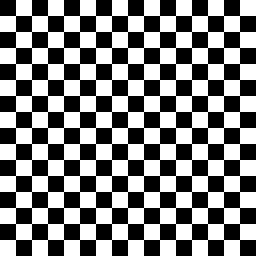
\includegraphics[width=1.25in]{figures/checker.jpg}  \\
\apiend


\apiitem{bool {\ce noise} (ImageBuf \&dst, string_view noisetype, \\
\bigspc\bigspc float A = 0.0f, float B = 0.1f, bool mono = false, \\
\bigspc\bigspc int seed = 0, ROI roi=ROI::All(), int nthreads=0)}
\indexapi{noise}
\NEW % 1.6

Add pseudorandom noise to the specified region of {\cf dst}. For noise
type \qkw{uniform}, the noise is uniformly distributed on the
range {\cf [A,B)]}. For noise \qkw{gaussian}, the noise will have a
normal distribution with mean A and standard deviation B.
For noise \qkw{salt}, the value A will be stored in a random set of pixels
whose proportion (of the overall image) is B.
For all noise types, choosing different {\cf seed} values will result in a

different pattern. If the {\cf mono} flag is {\cf true}, a single noise
value will be applied to all channels specified by {\cf roi}, but if {\cf
mono} is {\cf false}, a separate noise value will be computed for each channel in
the region.

If {\cf dst} is uninitialized, it will be resized to be a {\cf float}
\ImageBuf large enough to hold the region specified by {\cf roi}. It is an
error to pass both an uninitialized {\cf dst} and an undefined {\cf roi}.

\smallskip
\noindent Examples:
\begin{code}
    // Create a new 256x256 field of grayscale uniformly distributed noise on [0,1)
    ImageBuf A (ImageSpec(256, 256, 3, TypeDesc::FLOAT));
    ImageBufAlgo::zero (A);
    ImageBufAlgo::noise (A, "uniform", 0.0f /*min*/, 1.0f /*max*/,
                         true /*mono*/, 1 /*seed*/);

    // Add color Gaussian noise to an existing image
    ImageBuf B ("tahoe.jpg");
    ImageBufAlgo::noise (B, "gaussian", 0.0f /*mean*/, 0.1f /*stddev*/,
                         false /*mono*/, 1 /*seed*/);

    // Use salt and pepper noise to make occasional random dropouts
    ImageBuf C ("tahoe.jpg");
    ImageBufAlgo::noise (C, "salt", 0.0f /*value*/, 0.01f /*portion*/,
                         true /*mono*/, 1 /*seed*/);
\end{code}

\spc 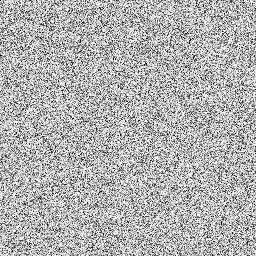
\includegraphics[width=1.25in]{figures/unifnoise1.jpg}
\spc 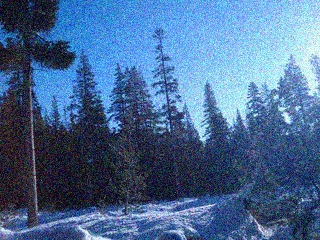
\includegraphics[width=1.65in]{figures/tahoe-gauss.jpg} 
\spc 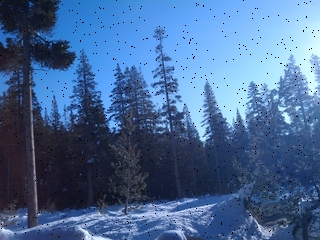
\includegraphics[width=1.65in]{figures/tahoe-pepper.jpg}

\apiend


\apiitem{bool {\ce render_text} (ImageBuf \&dst, int x, int y, string_view text,\\
  \bigspc\spc\spc int fontsize=16, string_view fontname="", \\
  \bigspc\spc\spc  const float *textcolor = NULL)}
\index{ImageBufAlgo!render_text} \indexapi{render_text}
Render a text string (encode as UTF-8) into the destination, essentially
doing an ``over'' of the antialiased character into the existing pixel data.
The baseline of the first character will start at position ({\cf x, y}).
The font is given by {\cf fontname} as a full pathname to the font file
(defaulting to some reasonable system font if not supplied at all), and with
a nominal height of {\cf fontsize} (in pixels).  The characters will be
drawn in opaque white (1.0 in all channels), unless {\cf textcolor} is
supplied (and is expected to point to a {\cf float} array of length at least
equal to the number of channels in {\cf dst}).

\smallskip
\noindent Examples:
\begin{code}
    ImageBuf A (ImageSpec (640, 480, 4, TypeDesc::FLOAT));

    ImageBufAlgo::render_text (A, 50, 100, "Hello, world");

    float red[] = { 1, 0, 0, 1 };
    ImageBufAlgo::render_text (A, 100, 200, "Go Big Red!",
                               60, "Arial Bold", red);
\end{code}
\spc 
\includegraphics[width=2.5in]{figures/text.jpg}  \\

\noindent Note that because of slightly differing fonts and versions of
Freetype available, we do not expect drawn text to be pixel-for-pixel 
identical on different platforms supported by \product.
\apiend





\section{Image transformations and data movement}
\label{sec:iba:transforms}

\apiitem{bool {\ce channels} (ImageBuf \&dst, const ImageBuf \&src, int nchannels, \\
        \bigspc  const int *channelorder,  const float *channelvalues=NULL, \\
        \bigspc                 const std::string *newchannelnames=NULL, \\
        \bigspc                 bool shuffle_channel_names=false)}
\index{ImageBufAlgo!channels} \indexapi{channels} \label{sec:iba:channels}

Generic channel shuffling: copy {\cf src} to {\cf dst}, but with channels in
the order specified by {\cf channelorder[0..nchannels-1]}.  Does not support in-place
operation.  For any channel in which {\cf channelorder[i]} $< 0$, it will
just make {\cf dst} channel {\cf i} be a constant value set to {\cf channelvalues[i]}
(if {\cf channelvalues} is not \NULL) or {\cf 0.0} (if {\cf channelvalues} is \NULL).

If {\cf channelorder} is \NULL, it will be interpreted as
{\cf \{0, 1, ..., nchannels-1\}}, meaning that it's only renaming channels,
not reordering them.

If {\cf newchannelnames} is not \NULL, it points to an array of new channel
names.  Channels for which {\cf newchannelnames[i]} is the empty string (or
all channels, if {\cf newchannelnames == NULL}) will be named as follows:
If {\cf shuffle_channel_names} is {\cf false}, the resulting dst image will have
default channel names in the usual order (\qkw{R}, \qkw{G}, etc.), but if
{\cf shuffle_channel_names} is {\cf true}, the names will be taken from the
corresponding channels of the source image -- be careful with this,
shuffling both channel ordering and their names could result in no
semantic change at all, if you catch the drift.

\smallskip
\noindent Examples:
\begin{code}
    // Copy the first 3 channels of an RGBA, drop the alpha
    ImageBuf RGBA (...);   // assume it's initialized, 4 chans
    ImageBuf RGB;
    ImageBufAlgo::channels (RGB, RGBA, 3, NULL /*default ordering*/);

    // Copy just the alpha channel, making a 1-channel image
    ImageBuf Alpha;
    int alpha_channel[] = { 3 /* alpha channel */ };
    ImageBufAlgo::channels (Alpha, RGBA, 1, &alpha_channel);

    // Swap the R and B channels
    ImageBuf BRGA;
    int channelorder[] = { 2 /*B*/, 1 /*G*/, 0 /*R*/, 3 /*A*/ };
    ImageBufAlgo::channels (BRGA, RGBA, 4, &channelorder);

    // Add an alpha channel with value 1.0 everywhere to an RGB image,
    // keep the other channels with their old ordering, values, and
    // names.
    int channelorder[] = { 0, 1, 2, -1 /*use a float value*/ };
    float channelvalues[] = { 0 /*ignore*/, 0 /*ignore*/, 0 /*ignore*/, 1.0 };
    std::string channelnames[] = { "", "", "", "A" };
    ImageBufAlgo::channels (RGBA, RGB, 4, channelorder,
                            channelvalues, channelnames);
\end{code}
\apiend

\apiitem{bool {\ce channel_append} (ImageBuf \&dst, const ImageBuf \&A, const ImageBuf \&B, \\
        \bigspc  ROI roi=ROI::All(), int nthreads=0)}
\index{ImageBufAlgo!channel_append} \indexapi{channel_append}
Append the channels of {\cf A} and {\cf B} together into {\cf dst} over
the region of interest.  If the region passed is uninitialized (the
default), it will be interpreted as being the union of the pixel windows
of {\cf A} and {\cf B} (and all channels of both images).  If {\cf dst}
is not already initialized, it will be resized to be big enough for the
region.

\smallskip
\noindent Examples:
\begin{code}
    ImageBuf RGBA (...);   // assume initialized, 4 channels
    ImageBuf Z (...);      // assume initialized, 1 channel
    ImageBuf RGBAZ;
    ImageBufAlgo::channel_append (RGBAZ, RGBA, Z);
\end{code}
\apiend


\apiitem{bool {\ce crop} (ImageBuf \&dst, const ImageBuf \&src, \\
        \bigspc  ROI roi=ROI::All(), int nthreads=0)}
\index{ImageBufAlgo!crop} \indexapi{crop}
Reset {\cf dst} to be the specified region of {\cf src}.

Note that the {\cf crop} operation does not actually move the pixels on the
image plane or adjust the full/display window; it merely restricts which
pixels are copied from {\cf src} to {\cf dst}.  (Note the difference
compared to {\cf cut()}).

\smallskip
\noindent Examples:
\begin{code}
    // Set B to be the upper left 200x100 region of A
    ImageBuf A (...);  // Assume initialized
    ImageBuf B;
    ImageBufAlgo::crop (B, A, ROI(0,200,0,100));
\end{code}
\apiend


\apiitem{bool {\ce cut} (ImageBuf \&dst, const ImageBuf \&src, \\
        \bigspc  ROI roi=ROI::All(), int nthreads=0)}
\index{ImageBufAlgo!cut} \indexapi{cut}
Reset {\cf dst} to be the specified region of {\cf src}, but repositioned at
the image plane origin and with the full/display window set to exactly cover
the new pixel window.  (Note the difference compared to {\cf crop()}).

\smallskip
\noindent Examples:
\begin{code}
    // Set B to be the 100x100 region of A with origin (50,200).
    ImageBuf A (...);  // Assume initialized
    ImageBuf B;
    ImageBufAlgo::cut (B, A, ROI(50,250,200,300));
    // Note: B has origin at 0,0, NOT at (50,200).
\end{code}
\apiend


\apiitem{bool {\ce paste} (ImageBuf \&dst, int xbegin, int ybegin, int zbegin,
  int chbegin, \\
  \bigspc const ImageBuf \&src, ROI srcroi=ROI::All(), int nthreads=0)}
\index{ImageBufAlgo!paste} \indexapi{paste}
Copy into {\cf dst}, beginning at {\cf (xbegin, ybegin, zbegin)}, the pixels of
{\cf src} described by {\cf srcroi}.  If {\cf srcroi} is {\cf ROI::All()},
the entirety of src will be used.  It will copy into channels 
{\cf [chbegin...]}, as many channels as are described by {\cf srcroi}.

\smallskip
\noindent Examples:
\begin{code}
    // Paste small.exr on top of big.exr at offset (100,100)
    ImageBuf Big ("big.exr");
    ImageBuf Small ("small.exr");
    ImageBufAlgo::paste (Big, 100, 100, 0, 0, Small);
\end{code}
\apiend


\apiitem{bool {\ce rotate90} (ImageBuf \&dst, const ImageBuf \&src, \\
        \bigspc  ROI roi=ROI::All(), int nthreads=0)}
\index{ImageBufAlgo!rotate90} \indexapi{rotate90}
Copy {\cf src} (or a subregion of {\cf src} to the corresponding pixels
of {\cf dst}, but rotated 90 degrees clockwise.

\smallskip
\noindent Examples:
\begin{code}
    ImageBuf A ("grid.jpg");
    ImageBuf B;
    ImageBufAlgo::rotate90 (B, A);
\end{code}
\spc 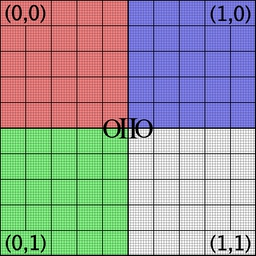
\includegraphics[width=1.25in]{figures/grid-small.jpg}
~ {\Huge $\rightarrow$} ~
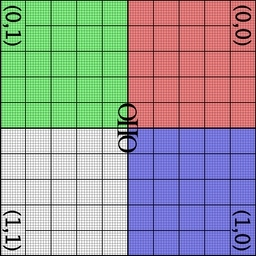
\includegraphics[width=1.25in]{figures/rotate90.jpg} \\
\apiend


\apiitem{bool {\ce rotate180} (ImageBuf \&dst, const ImageBuf \&src, \\
        \bigspc  ROI roi=ROI::All(), int nthreads=0)}
\index{ImageBufAlgo!rotate180} \indexapi{rotate180}
Copy {\cf src} (or a subregion of {\cf src} to the corresponding pixels
of {\cf dst}, but rotated 180 degrees.

\smallskip
\noindent Examples:
\begin{code}
    ImageBuf A ("grid.jpg");
    ImageBuf B;
    ImageBufAlgo::rotate180 (B, A);
\end{code}
\spc 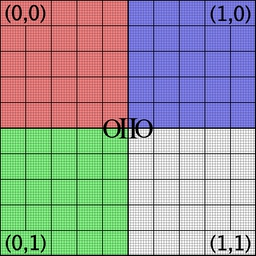
\includegraphics[width=1.25in]{figures/grid-small.jpg}
~ {\Huge $\rightarrow$} ~
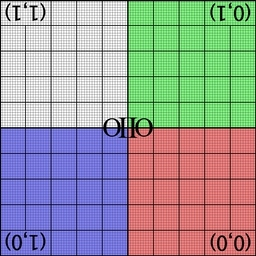
\includegraphics[width=1.25in]{figures/rotate180.jpg} \\
\apiend


\apiitem{bool {\ce rotate270} (ImageBuf \&dst, const ImageBuf \&src, \\
        \bigspc  ROI roi=ROI::All(), int nthreads=0)}
\index{ImageBufAlgo!rotate270} \indexapi{rotate270}
Copy {\cf src} (or a subregion of {\cf src} to the corresponding pixels
of {\cf dst}, but rotated 270 degrees clockwise (or 90 degrees
counter-clockwise).

\smallskip
\noindent Examples:
\begin{code}
    ImageBuf A ("grid.jpg");
    ImageBuf B;
    ImageBufAlgo::rotate270 (B, A);
\end{code}
\spc 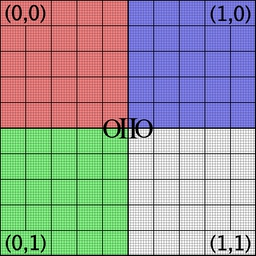
\includegraphics[width=1.25in]{figures/grid-small.jpg}
~ {\Huge $\rightarrow$} ~
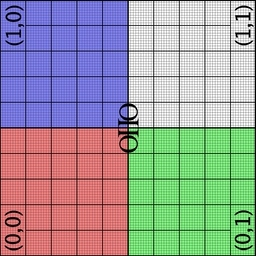
\includegraphics[width=1.25in]{figures/rotate270.jpg} \\
\apiend


\apiitem{bool {\ce flip} (ImageBuf \&dst, const ImageBuf \&src, \\
        \bigspc  ROI roi=ROI::All(), int nthreads=0)}
\index{ImageBufAlgo!flip} \indexapi{flip}
Copy {\cf src} (or a subregion of {\cf src}) to the corresponding pixels
of {\cf dst}, but with the scanlines exchanged vertically.

\smallskip
\noindent Examples:
\begin{code}
    ImageBuf A ("grid.jpg");
    ImageBuf B;
    ImageBufAlgo::flip (B, A);
\end{code}
\spc 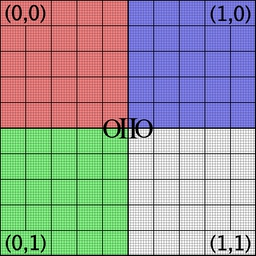
\includegraphics[width=1.25in]{figures/grid-small.jpg}
~ {\Huge $\rightarrow$} ~
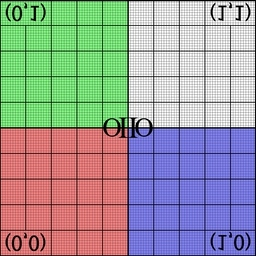
\includegraphics[width=1.25in]{figures/flip.jpg} \\
\apiend


\apiitem{bool {\ce flop} (ImageBuf \&dst, const ImageBuf \&src, \\
        \bigspc  ROI roi=ROI::All(), int nthreads=0)}
\index{ImageBufAlgo!flop} \indexapi{flop}
Copy {\cf src} (or a subregion of {\cf src}) to the corresponding pixels
of {\cf dst}, but with the columns exchanged horizontally.
\smallskip
\noindent Examples:
\begin{code}
    ImageBuf A ("grid.jpg");
    ImageBuf B;
    ImageBufAlgo::flop (B, A);
\end{code}
\spc 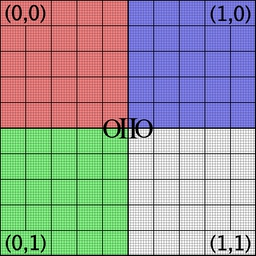
\includegraphics[width=1.25in]{figures/grid-small.jpg}
~ {\Huge $\rightarrow$} ~
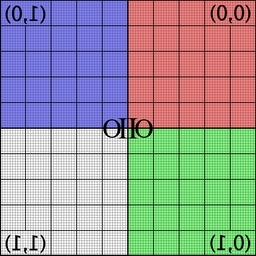
\includegraphics[width=1.25in]{figures/flop.jpg} \\
\apiend


\apiitem{bool {\ce reorient} (ImageBuf \&dst, const ImageBuf \&src, \\
        \bigspc  ROI roi=ROI::All(), int nthreads=0)}
\index{ImageBufAlgo!reorient} \indexapi{reorient}
Copy {\cf src} to {\cf dst}, but with whatever seties of rotations, flips,
or flops are necessary to transform the pixels into the configuration
suggested by the \qkw{Orientation} metadata of the image (and the
\qkw{Orientation} metadata is then set to 1, ordinary orientation).

It is allowed for {\cf src} and {\cf dst} to refer to the same image, in
which case the operation will be done ``in place'' (though not in a way
that is safe for another thread to be accessing the image simultaneously).

\smallskip
\noindent Examples:
\begin{code}
    ImageBuf A ("tahoe.jpg");
    ImageBufAlgo::reorient (A, A);
\end{code}
%\spc 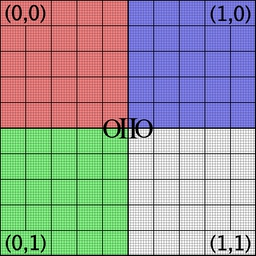
\includegraphics[width=1.25in]{figures/grid-small.jpg}
%~ {\Huge $\rightarrow$} ~
%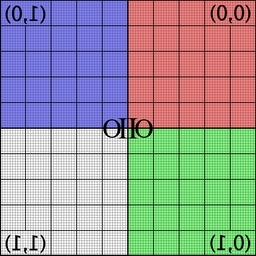
\includegraphics[width=1.25in]{figures/flop.jpg} \\
\apiend


\apiitem{bool {\ce transpose} (ImageBuf \&dst, const ImageBuf \&src, \\
        \bigspc  ROI roi=ROI::All(), int nthreads=0)}
\index{ImageBufAlgo!transpose} \indexapi{transpose}
Copy {\cf src} (or a subregion of {\cf src} to the corresponding 
transposed ($x \leftrightarrow y$) pixels
of {\cf dst}.  In other words, for all $(x,y)$ within the region,
set {\cf dst[y,x] = src[x,y]}.

\smallskip
\noindent Examples:
\begin{code}
    ImageBuf A ("grid.jpg");
    ImageBuf B;
    ImageBufAlgo::transpose (B, A);
\end{code}
\spc 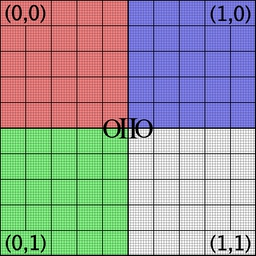
\includegraphics[width=1.25in]{figures/grid-small.jpg}
~ {\Huge $\rightarrow$} ~
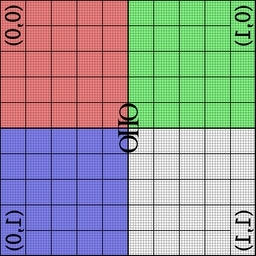
\includegraphics[width=1.25in]{figures/transpose.jpg} \\
\apiend


\apiitem{bool {\ce circular_shift} (ImageBuf \&dst, const ImageBuf \&src, \\
        \bigspc int xshift, int yshift, int zshift=0, \\
        \bigspc  ROI roi=ROI::All(), int nthreads=0)}
\index{ImageBufAlgo!circular_shift} \indexapi{circular_shift}

Copy {\cf src} (or a subregion of {\cf src} to the pixels of {\cf dst},
but circularly shifting by the given amount.  To clarify, the circular
shift of $[0,1,2,3,4,5]$ by $+2$ is $[4,5,0,1,2,3]$.

\smallskip
\noindent Examples:
\begin{code}
    ImageBuf A ("grid.jpg");
    ImageBuf B;
    ImageBufAlgo::circular_shift (B, A, 70, 30);
\end{code}
\spc 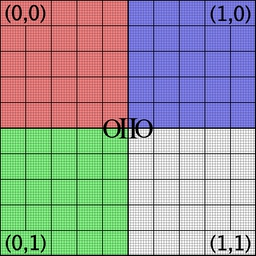
\includegraphics[width=1.25in]{figures/grid-small.jpg} 
~ {\Huge $\rightarrow$} ~
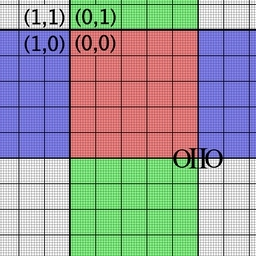
\includegraphics[width=1.25in]{figures/cshift.jpg} \\
\apiend


\apiitem{bool {\ce rotate} (ImageBuf \&dst, const ImageBuf \&src, \\
        \bigspc float angle, \\
        \bigspc string_view filtername="", float filtersize=0, \\
        \bigspc bool recompute_roi = false, \\
        \bigspc ROI roi=ROI::All(), int nthreads=0) \\
bool {\ce rotate} (ImageBuf \&dst, const ImageBuf \&src, \\
        \bigspc float angle, \\
        \bigspc Filter2D *filter, \\
        \bigspc bool recompute_roi = false, \\
        \bigspc ROI roi=ROI::All(), int nthreads=0) \\
bool {\ce rotate} (ImageBuf \&dst, const ImageBuf \&src, \\
        \bigspc float angle, float center_x, float center_y, \\
        \bigspc string_view filtername="", float filtersize=0, \\
        \bigspc bool recompute_roi = false, \\
        \bigspc ROI roi=ROI::All(), int nthreads=0) \\
bool {\ce rotate} (ImageBuf \&dst, const ImageBuf \&src, \\
        \bigspc float angle, float center_x, float center_y, \\
        \bigspc Filter2D *filter, \\
        \bigspc bool recompute_roi = false, \\
        \bigspc ROI roi=ROI::All(), int nthreads=0)}
\index{ImageBufAlgo!rotate} \indexapi{rotate}

Rotate the {\cf src} image by the {\cf angle} (in radians, with positive
angles clockwise). When {\cf center_x} and {\cf center_y} are supplied, they
denote the center of rotation; in their absence, the rotation will be about
the center of the image's display window.

Only the pixels (and channels) of {\cf dst} that are specified by {\cf roi}
will be copied from the rotated {\cf src}; the default {\cf roi} is to alter
all the pixels in {\cf dst}. If {\cf dst} is uninitialized, it will be
resized to be an ImageBuf large enough to hold the rotated image  if
{\cf recompute_roi} is {\cf true}, or will have the same ROI as {\cf src}
if {\cf recompute_roi} is false. It is an
error to pass both an uninitialied {\cf dst} and an undefined {\cf roi}.

The caller may explicitly pass a reconstruction filter, or specify one by
name and size, or if the name is the empty string {\cf rotate()} will choose
a reasonable high-quality default if \NULL is passed.  The filter is used to
weight the {\cf src} pixels falling underneath it for each {\cf dst} pixel;
the filter's size is expressed in pixel units of the {\cf dst} image.

\smallskip
\noindent Examples:
\begin{code}
    ImageBuf Src ("tahoe.exr");
    ImageBuf Dst;
    ImageBufAlgo::rotate (Dst, Src, 45.0);
\end{code}
\spc 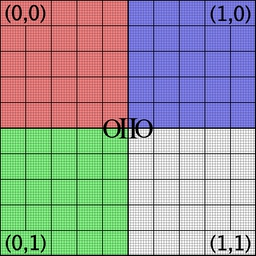
\includegraphics[width=1.25in]{figures/grid-small.jpg} 
~ {\Huge $\rightarrow$} ~
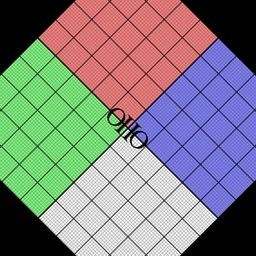
\includegraphics[width=1.25in]{figures/rotate45.jpg} \\
\apiend


\apiitem{bool {\ce warp} (ImageBuf \&dst, const ImageBuf \&src, \\
        \bigspc const Imath::M33f \&M, \\
        \bigspc string_view filtername="", float filtersize=0, \\
        \bigspc bool recompute_roi = false, \\
        \bigspc ImageBuf::WrapMode wrap = ImageBuf::WrapDefault, \\
        \bigspc ROI roi=ROI::All(), int nthreads=0) \\
bool {\ce warp} (ImageBuf \&dst, const ImageBuf \&src, \\
        \bigspc const Imath::M33f \&M, \\
        \bigspc Filter2D *filter, \\
        \bigspc bool recompute_roi = false, \\
        \bigspc ImageBuf::WrapMode wrap = ImageBuf::WrapDefault, \\
        \bigspc ROI roi=ROI::All(), int nthreads=0)}
\index{ImageBufAlgo!warp} \indexapi{warp}

Warp the {\cf src} image using the supplied 3x3 transformation matrix {\cf M}.

Only the pixels (and channels) of {\cf dst} that are specified by {\cf roi}
will be copied from the warped {\cf src}; the default {\cf roi} is to alter
all the pixels in {\cf dst}. If {\cf dst} is uninitialized, it will be
resized to be an \ImageBuf large enough to hold the warped image if
{\cf recompute_roi} is {\cf true}, or will have the same ROI as {\cf src}
if {\cf recompute_roi} is false. It is an
error to pass both an uninitialied {\cf dst} and an undefined {\cf roi}.

The caller may explicitly pass a reconstruction filter, or specify one by
name and size, or if the name is the empty string {\cf resize()} will choose
a reasonable high-quality default if \NULL is passed.  The filter is used to
weight the {\cf src} pixels falling underneath it for each {\cf dst} pixel;
the filter's size is expressed in pixel units of the {\cf dst} image.

\smallskip
\noindent Examples:
\begin{code}
    Imath::M33f M ( 0.7071068, 0.7071068, 0,
                   -0.7071068, 0.7071068, 0,
                   20,        -8.284271,  1);
    ImageBuf Src ("tahoe.exr");
    ImageBuf Dst;
    ImageBufAlgo::warp (dst, src, M, "lanczos3");
\end{code}
\apiend


\apiitem{bool {\ce resize} (ImageBuf \&dst, const ImageBuf \&src, \\
        \bigspc  string_view filtername="", float filtersize=0, \\
        \bigspc  ROI roi=ROI::All(), int nthreads=0) \\
bool {\ce resize} (ImageBuf \&dst, const ImageBuf \&src, \\
        \bigspc Filter2D *filter, \\
        \bigspc  ROI roi=ROI::All(), int nthreads=0)}
\index{ImageBufAlgo!resize} \indexapi{resize}
Set {\cf dst}, over the region of interest, to be a resized version of the
corresponding portion of {\cf src} (mapping such that the ``full'' image
window of each correspond to each other, regardless of resolution).  If
{\cf dst} is not yet initialized, it will be sized according to {\cf roi}.

The caller may explicitly pass a reconstruction filter, or specify one by
name and size, or if the name is the empty string {\cf resize()} will choose
a reasonable high-quality default if \NULL is passed.  The filter is used to
weight the {\cf src} pixels falling underneath it for each {\cf dst} pixel;
the filter's size is expressed in pixel units of the {\cf dst} image.

\smallskip
\noindent Examples:
\begin{code}
    // Resize the image to 640x480, using the default filter
    ImageBuf Src ("tahoe.exr");
    ImageBuf Dst;
    ROI roi (0, 640, 0, 480, 0, 1, /*chans:*/ 0, Src.nchannels());
    ImageBufAlgo::resize (Dst, Src, "", 0, roi);
\end{code}
\apiend


\apiitem{bool {\ce resample} (ImageBuf \&dst, const ImageBuf \&src, \\
        \bigspc bool interpolate = true, \\
        \bigspc ROI roi=ROI::All(), int nthreads=0)}
\index{ImageBufAlgo!resample} \indexapi{resample}
Set {\cf dst}, over the region of interest, to be a resized version of the
corresponding portion of {\cf src} (mapping such that the ``full'' image
window of each correspond to each other, regardless of resolution).  If
{\cf dst} is not yet initialized, it will be sized according to {\cf roi}.

Unlike {\cf ImageBufAlgo::resize()}, {\cf resample()} does not take a filter; it
just samples either with a bilinear interpolation (if {\cf interpolate} is
{\cf true}, the default) or uses the single ``closest'' pixel (if
{\cf interpolate} is {\cf false}).  This makes it a lot faster than a proper
{\cf resize()}, though obviously with lower quality (aliasing when
downsizing, pixel replication when upsizing).

\smallskip
\noindent Examples:
\begin{code}
    // Resample quickly to 320x240, using the default filter
    ImageBuf Src ("tahoe.exr");
    ImageBuf Dst;
    ROI roi (0, 320, 0, 240, 0, 1, /*chans:*/ 0, Src.nchannels());
    ImageBufAlgo::resample (Dst, Src, NULL, roi);
\end{code}
\apiend



\section{Image arithmetic}
\label{sec:iba:arith}

\apiitem{bool {\ce add} (ImageBuf \&dst, const ImageBuf \&A, const ImageBuf \&B, \\
        \bigspc  ROI roi=ROI::All(), int nthreads=0) \\
bool {\ce add} (ImageBuf \&dst, const ImageBuf \&A, float B, \\
        \bigspc ROI roi=ROI::All(), int nthreads=0) \\
bool {\ce add} (ImageBuf \&dst, const ImageBuf \&A, const float *B, \\
        \bigspc ROI roi=ROI::All(), int nthreads=0)}
\index{ImageBufAlgo!add} \indexapi{add}

For all pixels and channels within the designated region, set
{\cf dst} to the sum of image {\cf A} and {\cf B}.  {\cf B} is either an image,
a float (added to all channels) or a per-channel float array.
All of the images must have the same number of channels.

\smallskip
\noindent Examples:
\begin{code}
    // Add images A and B, assign to Sum
    ImageBuf A ("a.exr");
    ImageBuf B ("b.exr");
    ImageBuf Sum;
    ImageBufAlgo::add (Sum, A, B);

    // Add 0.2 to channels 0-2 of A
    ImageBuf A ("a.exr"), Sum;
    ROI roi = get_roi (A.spec());
    roi.chbegin = 0;  roi.chend = 3;
    ImageBufAlgo::add (Sum, A, 0.2, roi);
\end{code}
\apiend



\apiitem{bool {\ce sub} (ImageBuf \&dst, const ImageBuf \&A, const ImageBuf \&B, \\
        \bigspc  ROI roi=ROI::All(), int nthreads=0) \\
bool {\ce sub} (ImageBuf \&dst, const ImageBuf \&A, float B, \\
        \bigspc ROI roi=ROI::All(), int nthreads=0) \\
bool {\ce sub} (ImageBuf \&dst, const ImageBuf \&A, const float *B, \\
        \bigspc ROI roi=ROI::All(), int nthreads=0)}
\index{ImageBufAlgo!sub} \indexapi{sub}

For all pixels within the designated region, subtract {\cf B} from {\cf A},
putting the results into {\cf dst}. {\cf B} is either an image, a float
(added to all channels) or a per-channel float array. All of the images must
have the same number of channels.

\smallskip
\noindent Examples:
\begin{code}
    ImageBuf A ("a.exr");
    ImageBuf B ("b.exr");
    ImageBuf Difference;
    ImageBufAlgo::sub (Difference, A, B);
\end{code}
\apiend


\apiitem{bool {\ce absdiff} (ImageBuf \&dst, const ImageBuf \&A, const ImageBuf \&B, \\
        \bigspc  ROI roi=ROI::All(), int nthreads=0) \\
bool {\ce absdiff} (ImageBuf \&dst, const ImageBuf \&A, float B, \\
        \bigspc ROI roi=ROI::All(), int nthreads=0) \\
bool {\ce absdiff} (ImageBuf \&dst, const ImageBuf \&A, const float *B, \\
        \bigspc ROI roi=ROI::All(), int nthreads=0)}
\index{ImageBufAlgo!absdiff} \indexapi{absdiff}
\NEW % 1.6

For all pixels within the designated region, compute the absolute value of
the difference between the corresponding pixels of {\cf A} from {\cf B},
putting the results into {\cf dst}. {\cf A} is an \ImageBuf.  {\cf B} may be
an \ImageBuf (with the same number of channels as {\cf A}), or an array of
floats (one per channel, for each channel of {\cf A}), or a single float
(same value for all channels).

\smallskip
\noindent Examples:
\begin{code}
    ImageBuf A ("a.exr");
    ImageBuf B ("b.exr");
    ImageBuf Difference;
    ImageBufAlgo::absdiff (Difference, A, B);
\end{code}
\apiend


\apiitem{bool {\ce abs} (ImageBuf \&dst, const ImageBuf \&A, \\
        \bigspc  ROI roi=ROI::All(), int nthreads=0)}
\index{ImageBufAlgo!abs} \indexapi{abs}
\NEW % 1.6

For all pixels within the designated region, compute the absolute value of
the corresponding pixels of {\cf A}, putting the results into {\cf dst}.

\smallskip
\noindent Examples:
\begin{code}
    ImageBuf A ("a.exr");
    ImageBuf Abs;
    ImageBufAlgo::abs (Abs, A);
\end{code}
\apiend



\apiitem{bool {\ce mul} (ImageBuf \&dst, const ImageBuf \&A, const ImageBuf \&B, \\
        \bigspc  ROI roi=ROI::All(), int nthreads=0) \\
bool {\ce mul} (ImageBuf \&dst, const ImageBuf \&A, float B, \\
        \bigspc ROI roi=ROI::All(), int nthreads=0) \\
bool {\ce mul} (ImageBuf \&dst, const ImageBuf \&A, const float *B, \\
        \bigspc ROI roi=ROI::All(), int nthreads=0)}
\index{ImageBufAlgo!mul} \indexapi{mul}

For all pixels within the designated region, multiply the pixel values
of image {\cf A} by {\cf B} (channel by channel), putting the product in
{\cf dst}.  {\cf B} is either an image,
a float (added to all channels) or a per-channel float array.
All of the images must have the same number of channels.

\smallskip
\noindent Examples:
\begin{code}
    ImageBuf A ("a.exr");
    ImageBuf B ("b.exr");
    ImageBuf Product;
    ImageBufAlgo::mul (Product, A, B);

    // Reduce intensity of A's channels 0-2 by 50%
    ROI roi = get_roi (A.spec());
    roi.chbegin = 0;  roi.chend = 3;
    ImageBufAlgo::mul (A, A, 0.5, roi);
\end{code}
\apiend


\apiitem{bool {\ce div} (ImageBuf \&dst, const ImageBuf \&A, const ImageBuf \&B, \\
        \bigspc  ROI roi=ROI::All(), int nthreads=0) \\
bool {\ce div} (ImageBuf \&dst, const ImageBuf \&A, float B, \\
        \bigspc ROI roi=ROI::All(), int nthreads=0) \\
bool {\ce div} (ImageBuf \&dst, const ImageBuf \&A, const float *B, \\
        \bigspc ROI roi=ROI::All(), int nthreads=0)}
\index{ImageBufAlgo!div} \indexapi{div}
\NEW %1.6

For all pixels within the designated region, divide the pixel values
of image {\cf A} by {\cf B} (channel by channel), putting the result in
{\cf dst}.  {\cf B} is either an image,
a float (added to all channels) or a per-channel float array.
All of the images must have the same number of channels.
Division by zero is definied to result in zero.

\smallskip
\noindent Examples:
\begin{code}
    ImageBuf A ("a.exr");
    ImageBuf B ("b.exr");
    ImageBuf Result;
    ImageBufAlgo::div (Result, A, B);

    // Reduce intensity of A's channels 0-2 by 50%
    ROI roi = get_roi (A.spec());
    roi.chbegin = 0;  roi.chend = 3;
    ImageBufAlgo::div (A, A, 2.0f, roi);
\end{code}
\apiend


\apiitem{bool {\ce mad} (ImageBuf \&dst, const ImageBuf \&A, const ImageBuf \&B, \\
        \bigspc  const ImageBuf \&C, ROI roi=ROI::All(), int nthreads=0) \\
bool {\ce mad} (ImageBuf \&dst, const ImageBuf \&A, float B, \\
        \bigspc float C, ROI roi=ROI::All(), int nthreads=0) \\
bool {\ce mad} (ImageBuf \&dst, const ImageBuf \&A, const float *B, \\
        \bigspc const float *C, ROI roi=ROI::All(), int nthreads=0)}
\index{ImageBufAlgo!mad} \indexapi{mad}
\NEW % 1.6

For all pixels within the designated region, compute {\cf dst = A * B + C}
(pixel by pixel, channel by channel). {\cf A} must be an image. {\cf B} and
{\cf C} are either both images, both single floats (applied to all
channels), or are both per-channel float arrays. All of the images must have
the same number of channels.

\smallskip
\noindent Examples:
\begin{code}
    ImageBuf A ("a.exr");
    ImageBuf B ("b.exr");
    ImageBuf C ("c.exr");
    ImageBuf Result;
    ImageBufAlgo::mad (Result, A, B, C);

    // Compute the "inverse" A, which is 1.0-A, as A*(-1) + 1
    // Do this in-place, and only for the first 3 channels (leave any
    // alpha channel, if present, as it is).
    ROI roi = get_roi (A.spec());
    roi.chbegin = 0;  roi.chend = 3;
    ImageBufAlgo::mad (A, A, -1.0, 1.0, roi);
\end{code}
\apiend


\apiitem{bool {\ce invert} (ImageBuf \&dst, const ImageBuf \&A, \\
        \bigspc  ROI roi=ROI::All(), int nthreads=0)}
\index{ImageBufAlgo!invert} \indexapi{invert}
\NEW % 1.6

For all pixels and channels within the designated region, set {\cf dst}
to be the color inverse of the corresponding pixels of {\cf A}, that is,
1.0 - A.

\smallskip
\noindent Examples:
\begin{code}
    ImageBuf A ("a.exr");
    ImageBuf Inverse;
    ImageBufAlgo::invert (Inverse, A);

    // In this example, we are careful to deal with alpha in an RGBA
    // image. First we copy A to Inverse, and then in-place, we will:
    // un-premultiply the color values by alpha, invert just the color
    // channels, and then re-premultiply the colors by alpha.
    Inverse.copy (A);   // First copy A to inverse
    roi = A.roi();
    roi.chend = 3;      // Restrict roi to only R,G,B
    ImageBufAlgo::unpremult (Inverse, Inverse);
    ImageBufAlgo::invert (Inverse, Inverse, roi);
    ImageBufAlgo::premult (Inverse, Inverse);
\end{code}

%\spc 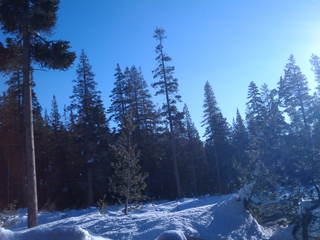
\includegraphics[width=1.5in]{figures/tahoe-small.jpg}
%\raisebox{40pt}{\large $\rightarrow$}
%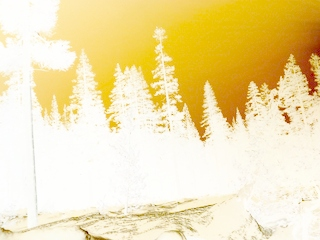
\includegraphics[width=1.5in]{figures/invert.jpg} \\
\apiend


\apiitem{bool {\ce pow} (ImageBuf \&dst, const ImageBuf \&A, float b, \\
        \bigspc ROI roi=ROI::All(), int nthreads=0) \\
bool {\ce pow} (ImageBuf \&dst, const ImageBuf \&A, const float *b, \\
        \bigspc ROI roi=ROI::All(), int nthreads=0)}
\index{ImageBufAlgo!pow} \indexapi{pow}

For all pixels within the designated region, raise the pixel value to the
power {\cf b} (channel by channel), putting the result in
{\cf dst}.  The value {\cf b} is either a single 
float (applied to all channels) or a per-channel float array.

\smallskip
\noindent Examples:
\begin{code}
    // Gamma-correct by 2.2 channels 0-2 of the image
    ROI roi = get_roi (A.spec());
    roi.chbegin = 0;  roi.chend = 3;
    ImageBufAlgo::mul (A, A, 1.0f/2.2f, roi);
\end{code}
\apiend


\apiitem{bool {\ce channel_sum} (ImageBuf \&dst, const ImageBuf \&src, \\
        \bigspc\spc const float *weights=NULL, \\
        \bigspc\spc ROI roi=ROI::All(), int nthreads=0)}
\index{ImageBufAlgo!channel_sum} \indexapi{channel_sum}
Converts a multi-channel image into a 1-channel image via a weighted sum
of channels.  For each pixel of {\cf src} within the designated ROI
(defaulting to all of {\cf src}, if not defined), sum the channels
designated by {\cf roi} and store the result in channel 0 of {\cf dst}.
If {\cf weights} is not \NULL, {\cf weight[i]} will provide a
per-channel weight (rather than defaulting to 1.0 for each channel).

\smallskip
\noindent Examples:
\begin{code}
    // Compute luminance via a weighted sum of R,G,B
    // (assuming Rec709 primaries and a linear scale)
    float luma_weights[3] = { .2126, .7152, .0722 };
    ImageBuf A ("a.exr");
    ImageBuf B;
    ROI roi = A.roi();
    roi.chbegin = 0;  roi.chend = 3;
    ImageBufAlgo::channel_sum (B, A, luma_weights, roi);
\end{code}
\apiend


\apiitem{bool {\ce clamp} (ImageBuf \&dst, const ImageBuf \&src, \\
  \bigspc float min = -std::numeric_limits<float>::max(), \\
  \bigspc float max = std::numeric_limits<float>::max(), \\
  \bigspc bool clampalpha01 = false, ROI roi=ROI::All(), int nthreads=0) \\
bool {\ce clamp} (ImageBuf \&dst, const ImageBuf \&src, \\
  \bigspc const float *min = NULL, const float *max = NULL, \\
  \bigspc bool clampalpha01 = false, ROI roi=ROI::All(), int nthreads=0)}
\index{ImageBufAlgo!clamp} \indexapi{clamp}

Copy pixels from {\cf src} to {\cf src} (within the {\cf roi}), clamping
between the {\cf min} and {\cf max} values.  Additionally, if
{\cf clampalpha01} is {\cf true}, then any alpha 
channel is clamped to the 0--1 range.

For the variety of {\cf clamp()} in which the {\cf min} and {\cf max}
values are {\cf float}, the minimum and maximum will be applied to
all color channels (or, at least, the subset of channels specified by
{\cf roi}).

For the variety of {\cf clamp()} in which the {\cf min} and {\cf max}
parameters are pointers, they point to arrays giving per-channel minimum
and maximum clamp values.  If {\cf min} is \NULL, no minimum clamping is
performed, and if {\cf max} is \NULL, no maximum clamping is performed.

\smallskip
\noindent Examples:
\begin{code}
    // Clamp image buffer A in-place to the [0,1] range for all pixels.
    ImageBufAlgo::clamp (A, A, 0.0f, 1.0f);

    // Just clamp alpha to [0,1]
    ImageBufAlgo::clamp (A, A, -std::numeric_limits<float>::max(),
                         std::numeric_limits<float>::max(), true);

    // Clamp R & G to [0,0.5], leave other channels alone
    std::vector<float> min (A.nchannels(), -std::numeric_limits<float>::max());
    std::vector<float> max (A.nchannels(), std::numeric_limits<float>::max());
    min[0] = 0.0f;  max[0] = 0.5f;
    min[1] = 0.0f;  max[1] = 0.5f;
    ImageBufAlgo::clamp (A, A, &min[0], &max[0], false);
\end{code}
\apiend


\apiitem{bool {\ce rangecompress} (ImageBuf \&dst, const ImageBuf \&src, bool useluma = false, \\
        \bigspc\bigspc  ROI roi=ROI::All(), int nthreads=0) \\
bool {\ce rangeexpand} (ImageBuf \&dst, const ImageBuf \&src, bool useluma = false, \\
        \bigspc\bigspc  ROI roi=ROI::All(), int nthreads=0)}
\index{ImageBufAlgo!rangecompress} \indexapi{rangecompress}
\index{ImageBufAlgo!rangeexpand} \indexapi{rangeexpand}

Some image operations (such as resizing with a ``good'' filter that
contains negative lobes) can have objectionable artifacts when applied
to images with very high-contrast regions involving extra bright pixels
(such as highlights in HDR captured or rendered images).  One way to
address this is by compressing the range of pixel values, then
performing the operation (such as a resize), then re-expanding the range
of the result again.  This approach can yield results that are much more
pleasing (even if not exactly mathematically correct).

The {\cf rangecompress} operation does the following: For all pixels and
color channels of {\cf src} within region {\cf roi} (defaulting to all
the defined pixels of {\cf src}), copy the pixels to {\cf dst}
while applying a logarithmic transformation on
their values.  Alpha and z channels are copied but not transformed.

The {\cf rangeexpand} operation is the opposite of {\cf rangecompress}: it
copies while rescaling the logarithmic color channel values back to a linear
response.

If {\cf useluma} is true, the luma of the first three channels (presumed
to be R, G, and B) are used to compute a single scale factor for all
color channels, rather than scaling all channels individually (which
could result in a big color shift when performing {\cf rangecompress}
and {\cf rangeexpand}).

\smallskip
\noindent Examples:
\begin{code}
    // Resize the image to 640x480, using a Lanczos3 filter, which
    // has negative lobes. To prevent those negative lobes from
    // producing ringing or negative pixel values for HDR data,
    // do range compression, then resize, then re-expand the range.

    // 1. Read the original image
    ImageBuf Src ("tahoeHDR.exr");

    // 2. Range compress to a logarithmic scale
    ImageBuf Compressed;
    ImageBufAlgo::rangecompress (Compressed, Src);

    // 3. Now do the resize
    ImageBuf Dst;
    ROI roi (0, 640, 0, 480, 0, 1, /*chans:*/ 0, Compressed.nchannels());
    ImageBufAlgo::resize (Dst, Comrpessed, "lanczos3", 6.0, roi);

    // 4. Expand range to be linear again (operate in-place)
    ImageBufAlgo::rangeexpand (Dst, Dst);
\end{code}
\apiend


\apiitem{bool {\ce over} (ImageBuf \&dst, const ImageBuf \&A, const ImageBuf \&B, \\
        \bigspc  ROI roi=ROI::All(), int nthreads=0)}
\index{ImageBufAlgo!over} \indexapi{over}

For all pixels within the designated region, combine the pixels of
images {\cf A} and {\cf B} using the Porter-Duff ``over'' compositing
operation, putting the result in {\cf dst}.  Image {\cf A} is the
``foreground,'' and {\cf B} is the ``background.''  Images {\cf A} and
{\cf B} must have the same number of channels and must both have an
alpha channel.

\smallskip
\noindent Examples:
\begin{code}
    ImageBuf A ("fg.exr");
    ImageBuf B ("bg.exr");
    ImageBuf Composite;
    ImageBufAlgo::over (Composite, A, B);
\end{code}
\apiend


\apiitem{bool {\ce zover} (ImageBuf \&dst, const ImageBuf \&A, const ImageBuf \&B, \\
        \bigspc  bool z_zeroisinf = false, ROI roi=ROI::All(), int nthreads=0)}
\index{ImageBufAlgo!zover} \indexapi{zover}

For all pixels within the designated region, combine the pixels of
images {\cf A} and {\cf B} using the Porter-Duff ``over'' compositing
operation, putting the result in {\cf dst}.  {\cf A} and {\cf B} must
have the same number of channels and must both alpha and $z$ (depth)
channels. Rather than {\cf A} always being the foreground (as it would
be for the {\cf over()} function, the $z$ channel is used to select
which image is foreground and which is background for each pixel
separately, with a lower $z$ value being the foreground for that pixel.
If {\cf z_zeroisinf} is {\cf true}, then $z=0$ values will be treated
as if they are infinitely far away.

\smallskip
\noindent Examples:
\begin{code}
    ImageBuf A ("a.exr");
    ImageBuf B ("b.exr");
    ImageBuf Composite;
    ImageBufAlgo::zover (Composite, A, B);
\end{code}
\apiend


\section{Image comparison and statistics}
\label{sec:iba:stats}

\apiitem{bool {\ce computePixelStats} (PixelStats \&stats, const ImageBuf \&src, \\
   \bigspc\bigspc  ROI roi=ROI::All(), int nthreads=0)}
\index{ImageBufAlgo!computePixelStats} \indexapi{computePixelStats}
\label{sec:iba:computePixelStats}

Compute statistics about the ROI of the image {\cf src}, storing results
in {\cf stats} (each of the vectors within {\cf stats} will be
automatically resized to the number of channels in the image).  A return
value of {\cf true} indicates success, {\cf false} indicates that it was
not possible to complete the operation.
 The {\cf PixelStats} structure is defined as follows:
\begin{code}
struct PixelStats {
    std::vector<float> min;
    std::vector<float> max;
    std::vector<float> avg;
    std::vector<float> stddev;
    std::vector<imagesize_t> nancount;
    std::vector<imagesize_t> infcount;
    std::vector<imagesize_t> finitecount;
    std::vector<double> sum, sum2;  // for intermediate calculation
};
\end{code}

\smallskip
\noindent Examples:
\begin{code}
    ImageBuf A ("a.exr");
    ImageBufAlgo::PixelStats stats;
    ImageBufAlgo::computePixelStats (stats, A);
    for (int c = 0;  c < A.nchannels();  ++c) {
        std::cout << "Channel " << c << ":\n";
        std::cout << "   min = " << stats.min[c] << "\n";
        std::cout << "   max = " << stats.max[c] << "\n";
        std::cout << "   average = " << stats.avg[c] << "\n";
        std::cout << "   standard deviation  = " << stats.stddev[c] << "\n";
        std::cout << "   # NaN values    = " << stats.nancount[c] << "\n";
        std::cout << "   # Inf values    = " << stats.infcount[c] << "\n";
        std::cout << "   # finite values = " << stats.finitecount[c] << "\n";
    }
\end{code}
\apiend

\apiitem{bool {\ce compare} (const ImageBuf \&A, const ImageBuf \&B, \\
  \bigspc float failthresh, float warnthresh, CompareResults \&result,\\
   \bigspc  ROI roi=ROI::All(), int nthreads=0)}
\index{ImageBufAlgo!compare} \indexapi{compare}

Numerically compare two images.  The difference threshold (for any
individual color channel in any pixel) for a ``failure'' is
{\cf failthresh}, and for a ``warning'' is {\cf warnthresh}.  The 
results are stored in {\cf result}.  If {\cf roi} is defined, pixels
will be compared for the pixel and channel range that is specified.  If
{\cf roi} is not defined, the comparison will be for all channels, on
the union of the defined pixel windows of the two images (for either
image, undefined pixels will be assumed to be black).  The 
{\cf CompareResults} structure is defined as follows:
\begin{code}
struct CompareResults {
    double meanerror, rms_error, PSNR, maxerror;
    int maxx, maxy, maxz, maxc;
    imagesize_t nwarn, nfail;
};
\end{code}

\smallskip
\noindent Examples:
\begin{code}
    ImageBuf A ("a.exr");
    ImageBuf B ("b.exr");
    ImageBufAlgo::CompareResults comp;
    ImageBufAlgo::compare (A, B, 1.0f/255.0f, 0.0f, comp);
    if (comp.nwarn == 0 && comp.nfail == 0) {
        std::cout << "Images match within tolerance\n";
    } else {
        std::cout << "Image differed: " << comp.nfail << " failures, "
                  << comp.nwarn << " warnings.\n";
        std::cout << "Average error was " << comp.meanerror << "\n";
        std::cout << "RMS error was " << comp.rms_error << "\n";
        std::cout << "PSNR was " << comp.PSNR << "\n";
        std::cout << "largest error was " << comp.maxerror 
                  << " on pixel (" << comp.maxx << "," << comp.maxy 
                  << "," << comp.maxz << "), channel " << comp.maxc << "\n";
    }
\end{code}
\apiend


\begin{comment}
 compare_Yee is a bit half-baked. Leave it out of the
  docs for now.  FIXME

\apiitem{int {\ce compare_Yee} (const ImageBuf \&A, const ImageBuf \&B, \\
  \bigspc CompareResults \&result, float luminance, float fov, \\
   \bigspc  ROI roi=ROI::All(), int nthreads=0)}
\index{ImageBufAlgo!compare_Yee} \indexapi{compare_Yee}
\apiend
\end{comment}


\apiitem{bool {\ce isConstantColor} (const ImageBuf \&src, float *color, \\
 \bigspc\bigspc         ROI roi=ROI::All(), int nthreads=0)}
\index{ImageBufAlgo!isConstantColor} \indexapi{isConstantColor}

If all pixels of {\cf src} within the ROI have the same values (for the
subset of channels described by {\cf roi}), return {\cf true} and store
the values in {\cf color[roi.chbegin...roi.chend-1]}.  Otherwise, return
{\cf false}.

\smallskip
\noindent Examples:
\begin{code}
    ImageBuf A ("a.exr");
    std::vector<float> color (A.nchannels());
    if (ImageBufAlgo::isConstantColor (A, &color[0])) {
        std::cout << "The image has the same value in all pixels: ";
        for (int c = 0;  c < A.nchannels();  ++c)
            std::cout << (c ? " " : "") << color[c];
        std::cout << "\n";
    } else {
        std::cout << "The image is not a solid color.\n";
    }
\end{code}
\apiend


\apiitem{bool {\ce isConstantChannel} (const ImageBuf \&src, int channel, float val, \\
 \bigspc\bigspc         ROI roi=ROI::All(), int nthreads=0)}
\index{ImageBufAlgo!isConstantChannel} \indexapi{isConstantChannel}

Returns {\cf true} if all pixels of {\cf src} within the ROI have the
given {\cf channel} value {\cf val}.

\smallskip
\noindent Examples:
\begin{code}
    ImageBuf A ("a.exr");
    int alpha = A.spec().alpha_channel;
    if (alpha < 0)
        std::cout << "The image does not have an alpha channel\n";
    else if (ImageBufAlgo::isConstantChannel (A, alpha, 1.0f))
        std::cout << "The image has alpha = 1.0 everywhere\n";
    else
        std::cout << "The image has alpha < 1 in at least one pixel\n";
\end{code}
\apiend

\apiitem{bool {\ce isMonochrome} (const ImageBuf \&src, 
          ROI roi=ROI::All(), int nthreads=0)}
\index{ImageBufAlgo!isMonochrome} \indexapi{isMonochrome}

Returns {\cf true} if the image is monochrome within the ROI, that is,
for all pixels within the region, do all channels 
{\cf [roi.chbegin, roi.chend)}
have the same value?  If roi is not defined (the default), it will be
understood to be all of the defined pixels and channels of source.

\smallskip
\noindent Examples:
\begin{code}
    ImageBuf A ("a.exr");
    ROI roi = get_roi (A.spec());
    roi.chend = std::min (3, roi.chend);  // only test RGB, not alpha
    if (ImageBufAlgo::isMonochrome (A, roi))
        std::cout << "a.exr is really grayscale\n";
\end{code}
\apiend


\apiitem{bool {\ce color_count} (const ImageBuf \&src, imagesize_t *count,\\
        \bigspc  int ncolors, const float *color, const float *eps=NULL,  \\
        \bigspc  ROI roi=ROI::All(), int nthreads=0)}
\index{ImageBufAlgo!color_count} \indexapi{color_count}

Count how many pixels in the image (within the ROI) match a list of colors.
The colors to match are in:

\begin{code}
  colors[0 ... nchans-1]
  colors[nchans ... 2*nchans-1]
  ...
  colors[(ncolors-1)*nchans ... (ncolors*nchans)-1]
\end{code}

\noindent and so on, a total of {\cf ncolors} consecutively stored
colors of {\cf nchans} channels each ({\cf nchans} is the number of
channels in the image, itself, it is not passed as a parameter).


The values in {\cf eps[0..nchans-1]} are the error tolerances for a
match, for each channel.  Setting {\cf eps[c]} to 
{\cf numeric_limits<float>::max()} will effectively make it ignore the
channel.  Passing {\cf eps == NULL} will be interpreted as a tolerance
of 0.001 for all channels (requires exact matches for 8 bit images, but
allows a wee bit of imprecision for {\cf float} images.

\smallskip
\noindent Examples:
\begin{code}
    ImageBuf A ("a.exr");
    int n = A.nchannels();

    // Try to match two colors: pure red and green
    std::vector<float> colors (2*n, numeric_limits<float>::max());
    colors[0] = 1.0f; colors[1] = 0.0f; colors[2] = 0.0f;
    colors[n+0] = 0.0f; colors[n+1] = 1.0f; colors[n+2] = 0.0f;

    const int ncolors = 2;
    imagesize_t count[ncolors];
    ImageBufAlgo::color_count (A, count, ncolors);
    std::cout << "Number of red pixels   : " << count[0] << "\n";
    std::cout << "Number of green pixels : " << count[1] << "\n";
\end{code}
\apiend


\apiitem{bool {\ce color_range_check} (const ImageBuf \&src, 
   imagesize_t *lowcount, \\ \bigspc imagesize_t *highcount, imagesize_t
  *inrangecount, \\
  \bigspc const float *low, const float *high, \\
        \bigspc  ROI roi=ROI::All(), int nthreads=0)}
\index{ImageBufAlgo!color_range_check} \indexapi{color_range_check}

Count how many pixels in the image (within the ROI) are outside the
value range described by {\cf low[roi.chbegin..roi.chend-1]} and
{\cf high[roi.chbegin..roi.chend-1]} 
as the low and high acceptable values for each color channel.  

The number of pixels containing values that fall below the lower bound
will be stored in {\cf *lowcount}, the number of pixels containing
values that fall above the upper bound will be stored in 
{\cf *highcount}, and the number of pixels for which all channels fell
within the bounds will be stored in {\cf *inrangecount}.  Any of these
may be NULL, which simply means that the counts need not be collected or
stored.

\smallskip
\noindent Examples:
\begin{code}
    ImageBuf A ("a.exr");
    ROI roi = get_roi (A.spec());
    roi.chend = std::min (roi.chend, 4);  // only compare RGBA

    float low[] = {0, 0, 0, 0};
    float high[] = {1, 1, 1, 1};

    imagesize_t lowcount, highcount, inrangecount;
    ImageBufAlgo::color_range_check (A, &lowcount, &highcount, &inrangecount,
                                     low, high, roi);
    std::cout << lowcount << " pixels had components < 0\n";
    std::cout << highcount << " pixels had components > 1\n";
    std::cout << inrangecount << " pixels were fully within [0,1] range\n";
\end{code}
\apiend


\apiitem{ROI {\ce nonzero_region} (const ImageBuf \&src, ROI roi=ROI::All(), int nthreads=0)}
\index{ImageBufAlgo!nonzero_region} \indexapi{nonzero_region}

Find the minimal rectangular region within {\cf roi} (which defaults to
the entire pixel data window of {\cf src}) that consists of nonzero pixel
values.  In other words, gives the region that is a ``shrink-wraps''
of {\cf src} to exclude black border pixels.  Note that if the entire
image was black, the ROI returned will contain no pixels.

For ``deep'' images, this function returns the smallest ROI that contains
all pixels that contain depth samples, and excludes the border pixels
that contain no depth samples at all.

\smallskip
\noindent Examples:
\begin{code}
    ImageBuf A ("a.exr");
    ROI shrunk = ImageBufAlgo::nonzero_region (A);
    if (shrunk.undefined())
        std::cout << "All pixels were empty\n";
    else
        std::cout << "Non-empty region was " << shrunk << "\n";
\end{code}
\apiend


\apiitem{std::string {\ce computePixelHashSHA1} (const ImageBuf \&src, \\
  \bigspc\bigspc string_view extrainfo = "", \\
  \bigspc\bigspc  ROI roi=ROI::All(), int blocksize=0, int nthreads=0)}
\index{ImageBufAlgo!computePixelHashSHA1} \indexapi{computePixelHashSHA1}

Compute the SHA-1 byte hash for all the pixels in the specifed region of
the image.  If {\cf blocksize} $> 0$, the function will compute separate
SHA-1 hashes of each {\cf blocksize} batch of scanlines, then return a
hash of the individual hashes.  This is just as strong a hash, but will
NOT match a single hash of the entire image ({\cf blocksize == 0}).  But
by breaking up the hash into independent blocks, we can parallelize
across multiple threads, given by {\cf nthreads}.
The {\cf extrainfo} provides additional text that will be
incorporated into the hash.

\smallskip
\noindent Examples:
\begin{code}
    ImageBuf A ("a.exr");
    std::string hash;
    hash = ImageBufAlgo::computePixelHashSHA1 (A, "", ROI::All(), 64);
\end{code}
\apiend

\apiitem{bool {\ce histogram} (const ImageBuf \&src, int channel, \\
  \bigspc std::vector<imagesize_t> \&histogram, int bins=256, \\
  \bigspc float min=0, float max=1, imagesize_t *submin=NULL, \\
  \bigspc imagesize_t *supermax=NULL, ROI roi=ROI::All())}
\index{ImageBufAlgo!histogram} \indexapi{histogram}
Computes a histogram of the given {\cf channel} of image {\cf src},
within the ROI,
as follows: The vector {\cf histogram[0..bins-1]} will contain the
count of pixels whose value was in each of the equally-sized range
bins between {\cf min} and {\cf max}; if {\cf submin} is not \NULL,
it specifies storage of the number of pixels whose value was
$<$ {\cf min}; if {\cf supermax} is not \NULL, it specifies storage of
the number of pixels whose value was $>$ {\cf max}.

\smallskip
\noindent Examples:
\begin{code}
    ImageBuf Src ("tahoe.exr");
    const int bins = 4;
    std::vector<imagesize_t> hist (bins, 0);
    imagesize_t submin=0, supermax=0;
    ImageBufAlgo::histogram (Src, 0, hist, bins, 0.0f, 1.0f,
                             &submin, &supermax);
    std::cout << "Channel 0 of the image had:\n";
    float binsize = (max-min)/nbins;
    for (int i = 0;  i < nbins;  ++i)
        hist[i] << " pixels that are >= " << (min+i*binsize) << " and "
                << (i == nbins-1 ? " <= " : " < ")
                << (min+(i+1)*binsize) << "\n";
    std::cout << submin << " pixels < " << min << "\n";
    std::cout << supermax << " pixels > " << max << "\n";
\end{code}
\apiend


\begin{comment}
% I'm not documenting histogram_draw at this point because as I started
% writing this section, I realized I really don't like this function 
% as it is written and would like to rewrite its specification when I
% get the chance.
\apiitem{bool {\ce histogram_draw} (ImageBuf \&dst, 
  \bigspc const std::vector<imagesize_t> \&histogram)}
\index{ImageBufAlgo!histogram_draw} \indexapi{histogram_draw}
\smallskip
\noindent Examples:
\begin{code}
\end{code}
\apiend
\end{comment}


\section{Convolutions}
\label{sec:iba:convolutions}

\apiitem{bool {\ce make_kernel} (ImageBuf \&dst, string_view name, \\
  \bigspc\spc float width, float height, float depth = 1.0f, \\
  \bigspc\spc                         bool normalize = true)}
\index{ImageBufAlgo!make_kernel} \indexapi{make_kernel}
Initialize {\cf dst} to be a 1-channel {\cf float} image of the named kernel.
The size of the {\cf dst} image will be big enough to contain the kernel
given its size ({\cf width} $\times$ {\cf height})
and rounded up to odd resolution so
that the center of the kernel can be at the center of the middle
pixel.  The kernel image will be offset so that its center is at the
{\cf (0,0)} coordinate.  If {\cf normalize} is true, the values will be
normalized so that they sum to $1.0$.

If {\cf depth} $> 1$, a volumetric kernel will be created.  Use with
caution!

Kernel names can be: \qkw{gaussian}, \qkw{sharp-gaussian}, \qkw{box},
\qkw{triangle}, \qkw{mitchell}, \qkw{blackman-harris}, \qkw{b-spline},
\qkw{catmull-rom}, \qkw{lanczos3}, \qkw{cubic}, \qkw{keys}, \qkw{simon},
\qkw{rifman}, \qkw{disk}, \qkw{binomial}. Note that
\qkw{catmull-rom} and \qkw{lanczos3} are fixed-size kernels that don't
scale with the width, and are therefore probably less useful in most
cases.

\smallskip
\noindent Examples:
\begin{code}
    ImageBuf K;
    ImageBufAlgo::make_kernel (K, "gaussian", 5.0f, 5.0f);
\end{code}
\apiend

\apiitem{bool {\ce convolve} (ImageBuf \&dst, const ImageBuf \&src, \\
  \bigspc const ImageBuf \&kernel, bool normalize = true, \\
  \bigspc  ROI roi=ROI::All(), int nthreads=0)}
\index{ImageBufAlgo!convolve} \indexapi{convolve}
Replace the given ROI of {\cf dst} with the convolution of {\cf src} and
a kernel.  If {\cf roi} is not defined, it defaults to the full size
of {\cf dst} (or {\cf src}, if {\cf dst} was uninitialized).
If {\cf dst} is uninitialized,
it will be allocated to be the size specified by {\cf roi}.  If 
{\cf normalized} is {\cf true}, the kernel will be normalized for the 
convolution, otherwise the original values will be used.

\smallskip
\noindent Examples:
\begin{code}
    // Blur an image with a 5x5 Gaussian kernel
    ImageBuf Src ("tahoe.exr");
    ImageBuf K;
    ImageBufAlgo::make_kernel (K, "gaussian", 5.0f, 5.0f);
    ImageBuf Blurred;
    ImageBufAlgo::convolve (Blurred, Src, K);
\end{code}

\spc \begin{tabular}{lll}
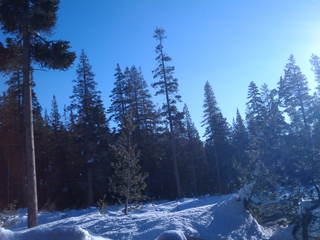
\includegraphics[width=1.5in]{figures/tahoe-small.jpg} &
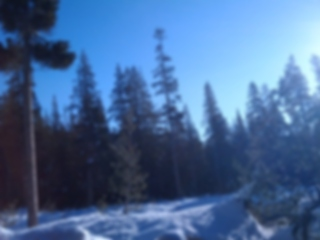
\includegraphics[width=1.5in]{figures/tahoe-blur.jpg} \\
original & blurred \\
\end{tabular}
\apiend

\apiitem{bool {\ce fft} (ImageBuf \&dst, const ImageBuf \&src, \\
        \bigspc  ROI roi=ROI::All(), int nthreads=0) \\
        bool {\ce ifft} (ImageBuf \&dst, const ImageBuf \&src, \\
        \bigspc  ROI roi=ROI::All(), int nthreads=0)}
\index{ImageBufAlgo!fft} \indexapi{fft}
\index{ImageBufAlgo!ifft} \indexapi{ifft}

The {\cf fft()} function takes the discrete Fourier transform (DFT) of
the section of {\cf src} denoted by {\cf roi}, storing it in {\cf dst}.
If {\cf roi} is not defined, it will be all of {\cf src}'s pixels.  Only
one channel of {\cf src} may be transformed at a time, so it will be the
first channel described by {\cf roi} (or, again, channel 0 if {\cf roi}
is undefined).  If not already in the correct format, {\cf dst} will be
re-allocated to be a 2-channel {\cf float} buffer of size 
{\cf roi.width()} $\times$ {\cf roi.height}, with channel 0 being the
``real'' part and channel 1 being the the ``imaginary'' part.  The
values returned are actually the unitary DFT, meaning that it is scaled
by $1/\sqrt{\mathrm{npixels}}$.

\smallskip
\noindent Examples:
\begin{code}
    ImageBuf Src ("tahoe.exr");

    // Take the DFT of the first channel of Src
    ImageBuf Freq;
    ImageBufAlgo::fft (Freq, Src);

    // At this point, Freq is a 2-channel float image (real, imag)
    // Convert it back from frequency domain to a spatial image
    ImageBuf Spatial;
    ImageBufAlgo::ifft (Spatial, Freq);
\end{code}
\apiend

\apiitem{bool {\ce complex_to_polar} (ImageBuf \&dst, const ImageBuf \&src, \\
        \bigspc  ROI roi=ROI::All(), int nthreads=0) \\
        bool {\ce polar_to_complex} (ImageBuf \&dst, const ImageBuf \&src, \\
        \bigspc  ROI roi=ROI::All(), int nthreads=0)}
\index{ImageBufAlgo!complex_to_polar} \indexapi{complex_to_polar}
\index{ImageBufAlgo!polar_to_complex} \indexapi{polar_to_complex}

The {\cf polar_to_complex()} function transforms a 2-channel image whose
channels are interpreted as complex values (real and imaginary components)
into the equivalent values expressed in polar form of amplitude and phase
(with phase between $0$ and $2\pi$).

The {\cf complex_to_polar()} function performs the reverse transformation,
converting from  polar values (amplitude and phase) to complex (real and
imaginary).

In either case,  the section of {\cf src} denoted by {\cf roi} is
transformed, storing the result in {\cf dst}. If {\cf roi} is not defined,
it will be all of {\cf src}'s pixels.  Only the first two channels of {\cf
src} will be transformed.

\smallskip
\noindent Examples:
\begin{code}
    // Suppose we have a set of frequency space values expressed as
    // amplitudes and phase...
    ImageBuf Polar ("polar.exr");

    // Convert to complex representation
    ImageBuf Complex;
    ImageBufAlgo::complex_to_polar (Complex, Polar);

    // Now, it's safe to take an IFFT of the complex image.
    // Convert it back from frequency domain to a spatial image.
    ImageBuf Spatial;
    ImageBufAlgo::ifft (Spatial, Complex);
\end{code}
\apiend



\section{Image Enhancement / Restoration}
\label{sec:iba:enhance}

\apiitem{bool {\ce fixNonFinite} (ImageBuf \&dst, const ImageBuf \&src, \\
  \bigspc\spc NonFiniteFixMode mode = NONFINITE_BOX3, \\
  \bigspc\spc int *pixelsFixed = NULL, \\
  \bigspc\spc  ROI roi=ROI::All(), int nthreads=0)}
\index{ImageBufAlgo!fixNonFinite} \indexapi{fixNonFinite}

Copy pixel values from {\cf src} to {\cf dst} (within the pixel and channel
range designated by {\cf roi}), and repair any non-finite ({\cf NaN} or {\cf
Inf}) pixels.  If {\cf pixelsFound} is not \NULL, store in it the number of
pixels that contained non-finite value.

How the non-finite values are repaired is specified by one of the
following modes:

\begin{description} 
\item[\spc] \spc
\item[\rm \kw{NONFINITE_NONE}]   do not alter the pixels (but do count the number
                       of nonfinite pixels in {\cf *pixelsFixed}, if non-\NULL).
\item[\rm \kw{NONFINITE_BLACK}]  change non-finite values to 0.
\item[\rm \kw{NONFINITE_BOX3}]   replace non-finite values by the average of any
                     finite pixels within a 3x3 window.
\end{description}

This works on all pixel data types, though it's just a copy for images with
pixel data types that cannot represent {\cf NaN} or {\cf Inf} values.


\smallskip
\noindent Examples:
\begin{code}
    ImageBuf Src ("tahoe.exr");
    int pixelsFixed = 0;
    ImageBufAlgo::fixNonFinite (Src, Src, ImageBufAlgo::NONFINITE_BOX3,
                                &pixelsFixed);
    std::cout << "Repaired " << pixelsFixed << " non-finite pixels\n";
\end{code}
\apiend


\apiitem{bool {\ce fillholes_pushpull} (ImageBuf \&dst, const ImageBuf \&src, \\
        \bigspc  ROI roi=ROI::All(), int nthreads=0)}
\index{ImageBufAlgo!fillholes_pushpull} \indexapi{fillholes_pushpull}
Copy the specified ROI of {\cf src} to {\cf dst} and fill any 
holes (pixels where alpha $< 1$) with plausible values using a push-pull
technique.  The {\cf src} image must have
an alpha channel.  The dst image will end up with a copy of src, but
will have an alpha of 1.0 everywhere, and any place where the alpha
of src was < 1, dst will have a pixel color that is a plausible
``filling'' of the original alpha hole.

\smallskip
\noindent Examples:
\begin{code}
    ImageBuf Src ("holes.exr");
    ImageBuf Filled;
    ImageBufAlgo::fillholes_pushpull (Filled, Src);
\end{code}
\apiend


\apiitem{bool {\ce median_filter} (ImageBuf \&dst, const ImageBuf \&src, \\
  \bigspc\spc int width = 3, int height = -1, \\
  \bigspc\spc  ROI roi=ROI::All(), int nthreads=0)}
\index{ImageBufAlgo!median_filter} \indexapi{median_filter}

Replace the given ROI of {\cf dst} with a median-filtered version of the
corresponding region of {\cf src}.  The median filter replaces each pixel
with the median value underneath the $\mathit{width} \times \mathit{height}$
window surrounding it. If the height is $< 1$, it will be set to width,
making a square window. The median filter tends to smooth out noise and
small high frequency details that are smaller than the window size, while
preserving the sharpness of long edges.

\smallskip
\noindent Examples:
\begin{code}
    ImageBuf Noisy ("tahoe.exr");
    ImageBuf Clean;
    ImageBufAlgo::median_filter (Clean, Noisy, 3, 3);
\end{code}

\spc \begin{tabular}{lll}
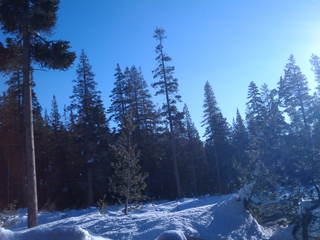
\includegraphics[width=1.5in]{figures/tahoe-small.jpg} &
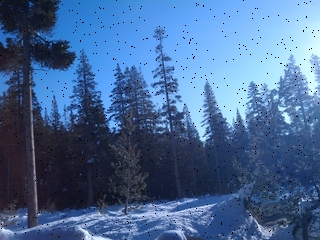
\includegraphics[width=1.5in]{figures/tahoe-pepper.jpg} &
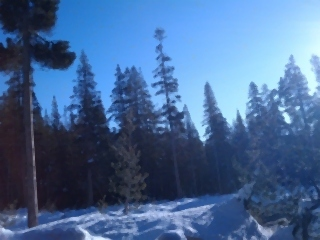
\includegraphics[width=1.5in]{figures/tahoe-pepper-median.jpg} \\
original & with dropouts & median filtered \\
\end{tabular}

\apiend


\apiitem{bool {\ce unsharp_mask} (ImageBuf \&dst, const ImageBuf \&src, \\
  \bigspc\spc string_view kernel = "gaussian", float width = 3.0f, \\
  \bigspc\spc float contrast = 1.0f, float threshold = 0.0f, \\
  \bigspc\spc  ROI roi=ROI::All(), int nthreads=0)}
\index{ImageBufAlgo!unsharp_mask} \indexapi{unsharp_mask}
\label{sec:iba:unsharpmask}

Replace the given ROI of {\cf dst} with a sharpened version of the
corresponding region of {\cf src} using the ``unsharp mask'' technique.
Unsharp masking basically works by first blurring the image (low
pass filter), subtracting this from the original image, then
adding the residual back to the original to emphasize the edges.
Roughly speaking,

\begin{code}
     dst = src + contrast * thresh(src - blur(src))
\end{code}

The specific blur can be selected by kernel name and width (for example,
\qkw{gaussian} is typical). As a special case, \qkw{median} is also accepted
as the kernel name, in which case a median filter is performed rather than
a blurring convolution (Gaussian and other blurs sometimes over-sharpen edges,
whereas using the median filter will sharpen compact high-frequency details
while not over-sharpening long edges).

The {\cf contrast} is a multiplier on the overall sharpening effect.  The
thresholding step causes all differences less than {\cf threshold} to be
squashed to zero, which can be useful for suppressing sharpening of
low-contrast details (like noise) but allow sharpening of
higher-contrast edges.

\smallskip
\noindent Examples:
\begin{code}
    ImageBuf Blurry ("tahoe.exr");
    ImageBuf Sharp;
    ImageBufAlgo::unsharp_mask (Sharp, Blurry, "gaussian", 5.0f);
\end{code}
\apiend


\section{Color manipulation}
\label{sec:iba:color}

\apiitem{bool {\ce colorconvert} (ImageBuf \&dst, const ImageBuf \&src, \\
  \bigspc\spc string_view from, string_view to, bool unpremult=false, \\
  \bigspc\spc ColorConfig *colorconfig=NULL, \\
  \bigspc\spc ROI roi=ROI::All(), int nthreads=0) \\
bool {\ce colorconvert} (ImageBuf \&dst, const ImageBuf \&src, \\
  \bigspc\spc const ColorProcessor *processor, bool unpremult=false, \\
  \bigspc\spc  ROI roi=ROI::All(), int nthreads=0)}
\index{ImageBufAlgo!colorconvert} \indexapi{colorconvert}
Copy pixels from {\cf src} to {\cf dst} (within the ROI), while
applying a color transform to the pixel values.
In-place operations ({\cf dst} and {\cf src} being the same image)
are supported.

If {\cf unpremult} is {\cf true}, unpremultiply before color conversion,
then premultiply again after the color conversion.  You may want to use
this flag if your image contains an alpha channel.

The first form of this function specifies the ``from'' and ``to'' color
spaces by name. An optional {\cf ColorConfig} is specified, but {\cf NULL}
is passed, the default OCIO color configuration found by examining the {\cf
\$OCIO} environment variable will be used instead.

The second form is directly passed a {\cf ColorProcessor}, which is is a
special object created by a {\cf ColorConfig} (see {\cf OpenImageIO/color.h}
for details).

If OIIO was built with OpenColorIO support enabled, then the transformation
may be between any two spaces supported by the active OCIO configuration, or
may be a ``look'' transformation created by {\cf
ColorConfig::createLookTransform}.  If OIIO was not built with OpenColorIO
support enabled, then the only transformations available are from \qkw{sRGB}
to \qkw{linear} and vice versa.

\smallskip
\noindent Examples:
\begin{code}
    #include <OpenImageIO/imagebufalgo.h>
    #include <OpenImageIO/color.h>
    using namespace OIIO;

    ImageBuf Src ("tahoe.jpg");
    ImageBuf Dst;
    ColorConfig cc;
    ColorProcessor *processor = cc.createColorProcessor ("vd8", "lnf");
    ImageBufAlgo::colorconvert (Dst, Src, processor, true);
    ColorProcessor::deleteColorProcessor (processor);

    // Equivalent, though possibly less efficient if you will be
    // converting many images using the same transformation:
    ImageBuf Src ("tahoe.jpg");
    ImageBuf Dst;
    ImageBufAlgo::colorconvert (Dst, Src, "vd8", "lnf", true);
\end{code}
\apiend

\apiitem{bool {\ce ociolook} (ImageBuf \&dst, const ImageBuf \&src, \\
  \bigspc\spc string_view looks, string_view from, string_view to, \\
  \bigspc\spc bool inverse=false, bool unpremult=false, \\
  \bigspc\spc string_view key="", string_view value="", \\
  \bigspc\spc ColorConfig *colorconfig=NULL, \\
  \bigspc\spc ROI roi=ROI::All(), int nthreads=0)}
\index{ImageBufAlgo!ociolook} \indexapi{ociolook}
Copy pixels from {\cf src} to {\cf dst} (within the ROI), while
applying an OpenColorIO ``look'' transform to the pixel values.
In-place operations ({\cf dst} and {\cf src} being the same image)
are supported.  The {\cf key} and {\cf value} may optionally be used
to establish a context (for example, a shot-specific transform).

If {\cf inverse} is {\cf true}, it will reverse the color transformation
and look application.

If {\cf unpremult} is {\cf true}, unpremultiply before color conversion,
then premultiply again after the color conversion.  You may want to use
this flag if your image contains an alpha channel.

An optional {\cf ColorConfig} is specified, but {\cf NULL} is passed, the
default OCIO color configuration found by examining the {\cf \$OCIO}
environment variable will be used instead.

\smallskip
\noindent Examples:
\begin{code}
    ImageBuf Src ("tahoe.jpg");
    ImageBuf Dst;
    ImageBufAlgo::ociolook (Dst, Src, "look", "vd8", "lnf", false, false,
                            "SHOT", "pe0012");
\end{code}
\apiend


\apiitem{bool {\ce ociodisplay} (ImageBuf \&dst, const ImageBuf \&src, \\
  \bigspc\spc string_view display, string_view view, \\
  \bigspc\spc string_view from="", string_view looks="",\\
  \bigspc\spc bool unpremult=false, \\
  \bigspc\spc string_view key="", string_view value="", \\
  \bigspc\spc ColorConfig *colorconfig=NULL, \\
  \bigspc\spc ROI roi=ROI::All(), int nthreads=0)}
\index{ImageBufAlgo!ociodisplay} \indexapi{ociodisplay}
Copy pixels from {\cf src} to {\cf dst} (within the ROI), while
applying an OpenColorIO ``display'' transform to the pixel values.
In-place operations ({\cf dst} and {\cf src} being the same image)
are supported.  If {\cf from} or {\cf looks} are empty, it will not
override the look or source color space (subtly different than
passing \qkw{}, the empty string, which means to use no look or source
space).  The {\cf key} and {\cf value} may optionally be used
to establish a context (for example, a shot-specific transform).

If {\cf inverse} is {\cf true}, it will reverse the color transformation
and look application.

If {\cf unpremult} is {\cf true}, unpremultiply before color conversion,
then premultiply again after the color conversion.  You may want to use
this flag if your image contains an alpha channel.

An optional {\cf ColorConfig} is specified, but {\cf NULL} is passed, the
default OCIO color configuration found by examining the {\cf \$OCIO}
environment variable will be used instead.

\smallskip
\noindent Examples:
\begin{code}
    ImageBuf Src ("tahoe.exr");
    ImageBuf Dst;
    ImageBufAlgo::ociodisplay (Dst, Src, "sRGB", "Film", "lnf", NULL,
                               false, "SHOT", "pe0012");
\end{code}
\apiend


\apiitem{bool {\ce unpremult} (ImageBuf \&dst, const ImageBuf \&src,\\
  \bigspc ROI roi=ROI::All(), int nthreads=0)}
\index{ImageBufAlgo!unpremult} \indexapi{unpremult}
Copy pixels from {\cf src} to {\cf dst}, and in the process 
divide all color channels (those not alpha or z) 
by the alpha value, to ``un-premultiply'' them.  This presumes that the
image starts of as ``associated alpha'' a.k.a.\ ``premultipled.''  The
alterations are restricted to the pixels and channels of the supplied
ROI (which defaults to all of {\cf src}).  Pixels in which the alpha
channel is 0 will not be modified (since the operation is undefined in
that case).  This is just a copy if there is no identified alpha channel
(and a no-op if {\cf dst} and {\cf src} are the same image).

\smallskip
\noindent Examples:
\begin{code}
    // Convert in-place from associated alpha to unassociated alpha
    ImageBuf A ("a.exr");
    ImageBufAlgo::unpremult (A, A);
\end{code}
\apiend

\apiitem{bool {\ce premult} (ImageBuf \&dst, const ImageBuf \&src, \\
  \bigspc ROI roi=ROI::All(), int nthreads=0)}
\index{ImageBufAlgo!premult} \indexapi{premult}
Copy pixels from {\cf src} to {\cf dst}, and in the process 
multiply all color channels (those not alpha or z) 
by the alpha value, to ``premultiply'' them.  This presumes that the
image starts of as ``unassociated alpha'' a.k.a.\ ``non-premultipled.''
The alterations are restricted to the pixels and channels of the
supplied ROI (which defaults to all of {\cf src}).  This is just a copy
if there is no identified alpha channel
(and a no-op if {\cf dst} and {\cf src} are the same image).

\smallskip
\noindent Examples:
\begin{code}
    // Convert in-place from unassociated alpha to associated alpha
    ImageBuf A ("a.exr");
    ImageBufAlgo::premult (A, A);
\end{code}
\apiend



\section{Import / export}
\label{sec:iba:importexport}

\apiitem{bool {\ce make_texture} (MakeTextureMode mode, const ImageBuf \&input, \\
\bigspc                             string_view outputfilename,
                             const ImageSpec \&config,\\
\bigspc                             std::ostream *outstream = NULL) \\
bool {\ce make_texture} (MakeTextureMode mode, string_view filename, \\
\bigspc                             string_view outputfilename,
                             const ImageSpec \&config,\\
\bigspc                             std::ostream *outstream = NULL)}
\index{ImageBufAlgo!make_texture} \indexapi{make_texture}

Turn an image file (either an existing \ImageBuf or specified by {\cf
filename}) into a tiled, MIP-mapped, texture file and write to the
file named by ({\cf outputfilename}).  The {\cf mode} describes what type of texture file we
are creating and may be one of the following:

\noindent \begin{tabular}{p{2in}p{3in}}
{\cf MakeTxTexture} & Ordinary 2D texture\\
%MakeTxShadow & \\
{\cf MakeTxEnvLatl} & Latitude-longitude environment map\\
{\cf \small MakeTxEnvLatlFromLightProbe} & Latitude-longitude environment map
       constructed from a ``light probe'' image.\\
\end{tabular}

If the {\cf outstream} pointer is not \NULL, it should point
to a stream (for example, {\cf \&std::out}, or a pointer to a local 
{\cf std::stringstream} to capture output), which is where console output
and error messages will be deposited.

The {\cf config} is an \ImageSpec that contains all the information and
special instructions for making the texture.  Anything set in {\cf config}
(format, tile size, or named metadata) will take precedence over
whatever is specified by the input file itself.  Additionally, named
metadata that starts with \qkw{maketx:} will not be output to the file
itself, but may contain instructions controlling how the texture is
created.  The full list of supported configuration options is:

\noindent Named fields:

\begin{tabular}{ >{\cf}l p{4in}}
   format         & Data format of the texture file (default: UNKNOWN =
                    same format as the input) \\
   tile_width     & \multirow{3}{*}{Preferred tile size (default: 64x64x1)} \\
   tile_height    &       \\
   tile_depth     & \\
\end{tabular}
\medskip

\noindent Metadata in {\cf config.extra_attribs}:

\begin{longtable}{ >{\spc \cf\small}p{1.8in} >{\cf\small}l p{3in}}
   compression & string &   Default: "zip" \\
   fovcot & float &          Default: aspect ratio of the image resolution \\
   planarconfig & string &  Default: "separate" \\
   worldtocamera & matrix &  World-to-camera matrix of the view. \\
   worldtoscreen & matrix &  World-to-screen space matrix of the view. \\
   wrapmodes & string &     Default: "black,black" \\
   maketx:verbose & int &    How much detail should go to outstream (0). \\
   maketx:stats & int &      If nonzero, print stats to outstream (0). \\
   maketx:resize & int &     If nonzero, resize to power of 2. (0) \\
   maketx:nomipmap & int &   If nonzero, only output the top MIP level (0). \\
   maketx:updatemode & int &  If nonzero, write new output only if the
                             output file doesn't already exist, or is
                             older than the input file. (0) \\
   \multicolumn{2}{l}{\spc \cf\small maketx:constant_color_detect} \\  & int &
                          If nonzero, detect images that are entirely
                            one color, and change them to be low
                            resolution (default: 0). \\
   \multicolumn{2}{l}{\spc \cf\small maketx:monochrome_detect} \\ & int &
                          If nonzero, change RGB images which have
                             R==G==B everywhere to single-channel
                             grayscale (default: 0). \\
   maketx:opaque_detect & int &
                          If nonzero, drop the alpha channel if alpha
                             is 1.0 in all pixels (default: 0). \\
   maketx:unpremult & int &  If nonzero, unpremultiply color by alpha before
                             color conversion, then multiply by alpha
                             after color conversion (default: 0). \\
   {\small maketx:incolorspace} & string & \\
   {\small maketx:outcolorspace} & string &
                          These two together will apply a color conversion
                              (with OpenColorIO, if compiled). Default: "" \\
   maketx:checknan & int &   If nonzero, will consider it an error if the
                              input image has any NaN pixels. (0) \\
   maketx:fixnan & string & If set to "black" or "box3", will attempt
                              to repair any NaN pixels found in the
                              input image (default: "none"). \\
   \multicolumn{2}{l}{\spc \cf\small maketx:set_full_to_pixels} \\ & int &
                          If nonzero, doctors the full/display window
                              of the texture to be identical to the
                              pixel/data window and reset the origin
                              to 0,0 (default: 0). \\
   maketx:filtername & string &
                          If set, will specify the name of a high-quality
                             filter to use when resampling for MIPmap
                             levels. Default: "", use bilinear resampling. \\
   maketx:highlightcomp & int &
                          If nonzero, performs highlight compensation --
                             range compression and expansion around 
                             the resize, plus clamping negative plxel
                             values to zero. This reduces ringing when
                             using filters with negative lobes. \\
   maketx:nchannels & int &  If nonzero, will specify how many channels
                             the output texture should have, padding with
                             0 values or dropping channels, if it doesn't
                             the number of channels in the input.
                             (default: 0, meaning keep all input channels) \\
   maketx:channelnames & string &
                          If set, overrides the channel names of the
                             output image (comma-separated). \\
   {\small maketx:fileformatname} & string &
                          If set, will specify the output file format.
                              (default: "", meaning infer the format from
                              the output filename) \\
   \multicolumn{2}{l}{\spc \cf\small maketx:prman_metadata} \\ & int &
                          If set, output some metadata that PRMan will
                              need for its textures. (0) \\
   {\small maketx:oiio_options} & int &
                          (Deprecated; all are handled by default) \\
   \multicolumn{2}{l}{\spc \cf\small maketx:prman_options} \\ & int &
                          If nonzero, override a whole bunch of settings 
                              as needed to make textures that are
                              compatible with PRMan. (0) \\
   maketx:mipimages & string &
                          Semicolon-separated list of alternate images
                              to be used for individual MIPmap levels,
                              rather than simply downsizing. (default: "") \\
   \multicolumn{2}{l}{\spc \cf\small maketx:full_command_line} \\ & string &
                          The command or program used to generate this
                              call, will be embedded in the metadata.
                              (default: "") \\
   \multicolumn{2}{l}{\spc \cf\small maketx:ignore_unassoc} \\ & int &
                          If nonzero, will disbelieve any evidence that
                              the input image is unassociated alpha. (0) \\
   \multicolumn{2}{l}{\spc \cf\small maketx:read_local_MB} \\ & int &
                          If nonzero, will read the full input file locally
                              if it is smaller than this threshold. Zero
                              causes the system to make a good guess at
                                a reasonable threshold (e.g. 1 GB). (0) \\
   maketx:forcefloat & int &
                          Forces a conversion through float data for
                              the sake of ImageBuf math. (1) \\
   maketx:hash & int &
                          Compute the sha1 hash of the file in parallel. (1) \\
   \multicolumn{2}{l}{\spc \cf\small maketx:allow_pixel_shift} \\ & int &
                          Allow up to a half pixel shift per mipmap level.
                              The fastest path may result in a slight shift
                              in the image, accumulated for each mip level
                              with an odd resolution. (0) \\
\end{longtable}

\smallskip
\noindent Examples:
\begin{code}
    // This command line:
    //    maketx in.exr --hicomp --filter lanczos3 --opaque-detect \
    //             -o texture.exr
    // is equivalent to:

    ImageBuf Input ("in.exr");
    ImageSpec config;
    config.attribute ("maketx:highlightcomp", 1);
    config.attribute ("maketx:filtername", "lanczos3");
    config.attribute ("maketx:opaquedetect", 1);
    stringstream s;
    bool ok = ImageBufAlgo::make_texture (ImageBufAlgo::MakeTxTexture,
                                          Input, "texture.exr", config, &s);
    if (! ok)
        std::cout << "make_texture error: " << s.str() << "\n";
\end{code}
\apiend


\apiitem{bool {\ce from_IplImage} (ImageBuf \&dst, const IplImage *ipl, \\
        \bigspc\bigspc  TypeDesc convert = TypeDesc::UNKNOWN)}
\index{ImageBufAlgo!from_IplImage} \indexapi{from_IplImage}
\index{OpenCV}\indexapi{IplImage}\index{Intel Image Library}
Convert an {\cf IplImage}, used by OpenCV and Intel's Image Libray, and
set {\cf dst} to be the same image (copying the pixels).  If {\cf convert} is
not set to {\cf UNKNOWN}, try to establish {\cf dst} as holding that
data type and convert the {\cf IplImage} data.  Return {\cf true} if ok,
{\cf false} if it couldn't figure out how to make the conversion from
{\cf IplImage} to an \ImageBuf.  If OpenImageIO was compiled without OpenCV
support, this function will return false without modifying {\cf dst}.

\begin{comment}
\smallskip
\noindent Examples:
\begin{code}
\end{code}
\end{comment}
\apiend


\apiitem{IplImage* {\ce to_IplImage} (const ImageBuf \&src)}
\index{ImageBufAlgo!to_IplImage} \indexapi{to_IplImage}
\index{OpenCV}\indexapi{IplImage}\index{Intel Image Library}
Construct an {\cf IplImage*}, used by OpenCV and Intel's Image Library,
that is equivalent to the \ImageBuf {\cf src}.  If it is not possible, or
if OpenImageIO was compiled without OpenCV support, then return
\NULL.  The ownership of the {\cf IplImage} is fully transferred to the
calling application.

\begin{comment}
\smallskip
\noindent Examples:
\begin{code}
\end{code}
\end{comment}
\apiend


\apiitem{bool {\ce capture_image} (ImageBuf \&dst, int cameranum, \\
        \bigspc\bigspc  TypeDesc convert = TypeDesc::UNKNOWN)}
\index{ImageBufAlgo!capture_image} \indexapi{capture_image}
Capture a still image from a designated camera.  If able to do so,
store the image in {\cf dst} and return {\cf true}.  If there is no such device,
or support for camera capture is not available (such as if OpenCV
support was not enabled at compile time), return {\cf false} and do not
alter {\cf dst}.

\smallskip
\noindent Examples:
\begin{code}
    ImageBuf WebcamImage;
    ImageBufAlgo::capture_image (WebcamImage, 0, TypeDesc::UINT8);
    WebcamImage.save ("webcam.jpg");
\end{code}
\apiend



\section{Deep images}
\label{sec:iba:deep}

A number of {\cf ImageBufAlgo} functions are designed to work with ``deep''
images. These are detailed below. In general, {\cf ImageBufAlgo} functions
not listed in this section should not be expected to work with deep images.

\subsection{Functions specific to deep images}

\apiitem{bool {\ce deepen} (ImageBuf \&dst, const ImageBuf \&src, float zvalue, \\
        \bigspc  ROI roi=ROI::All(), int nthreads=0)}
\index{ImageBufAlgo!deepen} \indexapi{deepen} \index{deep images}
\NEW % 1.6
Copy pixels from regular (not ``deep'') image {\cf src} into deep {\cf dst}.

If the {\cf src} image has a \qkw{Z} channel: if the source pixel's {\cf Z}
channel value is not infinite, the corresponding pixel of {\cf dst} will get
a single depth sample that copies the data from the soruce pixel; otherwise,
{\cf dst} will get an empty pixel. In other words, infinitely far pixels
will not turn into deep samples.

If the {\cf src} image lacks a \qkw{Z} channel: if any of the source pixel's
channel values are nonzero, the corresponding pixel of {\cf dst} will get a
single depth sample that copies the data from the source pixel and uses the
{\cf zvalue} parameter for the depth; otherwise, if all source channels in
that pixel are zero, the destination pixel will get no depth samples.

If {\cf src} is already a deep image, it will just copy pixel values from
{\cf src} to {\cf dst}. If {\cf dst} is not already an initialized
\ImageBuf, it will be sized to match {\cf src} (but made deep).

\smallskip
\noindent Examples:
\begin{code}
    ImageBuf Flat ("RGBAZ.exr");
    ImageBuf Deep;
    ImageBufAlgo::deepen (Deep, Flat);
\end{code}
\apiend

\apiitem{bool {\ce flatten} (ImageBuf \&dst, const ImageBuf \&src, \\
        \bigspc  ROI roi=ROI::All(), int nthreads=0)}
\index{ImageBufAlgo!flatten} \indexapi{flatten} \index{deep images}
Copy pixels from \emph{deep} image {\cf src} into non-deep {\cf dst},
compositing the depth samples within each pixel to yield a single ``flat''
value per pixel. If {\cf src} is not deep, it just copies the pixels without
alteration.

\smallskip
\noindent Examples:
\begin{code}
    ImageBuf Deep ("deepalpha.exr");
    ImageBuf Flat;
    ImageBufAlgo::flatten (Flat, Deep);
\end{code}
\apiend

\subsection{General functions that also work for deep images}

\apiitem{bool {\ce channels} (ImageBuf \&dst, const ImageBuf \&src, int nchannels, \\
        \bigspc  const int *channelorder,  const float *channelvalues=NULL, \\
        \bigspc                 const std::string *newchannelnames=NULL, \\
        \bigspc                 bool shuffle_channel_names=false)}
Reorder, rename, remove, or add channels to a deep image.
See Section~\ref{sec:iba:channels}
\apiend

\apiitem{bool {\ce computePixelStats} (PixelStats \&stats, const ImageBuf \&src, \\
   \bigspc\bigspc  ROI roi=ROI::All(), int nthreads=0)}
Compute per-channel statistics about the image.
See Section~\ref{sec:iba:computePixelStats}
\apiend

\apiitem{ROI {\ce nonzero_region} (const ImageBuf \&src, ROI roi=ROI::All(), int nthreads=0)}
\index{ImageBufAlgo!nonzero_region} \indexapi{nonzero_region}
For ``deep'' images, this function returns the smallest ROI that contains
all pixels that contain depth samples, and excludes the border pixels
that contain no depth samples at all.
\apiend

\apiitem{bool {\ce compare} (const ImageBuf \&A, const ImageBuf \&B, \\
  \bigspc float failthresh, float warnthresh, CompareResults \&result,\\
   \bigspc  ROI roi=ROI::All(), int nthreads=0)}
Numerically compare two images.
\apiend



\begin{comment}
\apiitem{bool {\ce blah} (ImageBuf \&dst, const ImageBuf \&src, \\
        \bigspc  ROI roi=ROI::All(), int nthreads=0)}
\index{ImageBufAlgo!blah} \indexapi{blah}
Blah.
\smallskip
\noindent Examples:
\begin{code}
\end{code}
\apiend
\end{comment}

\index{ImageBufAlgo|)}
\index{Image Processing|)}

\chapwidthend
